\documentclass[11pt]{report}
\usepackage[magyar]{babel}
\usepackage[utf8]{inputenc}
% \usepackage[T1]{fontenc}
%\usepackage{graphics}
\usepackage{graphicx}
\usepackage{amsmath}
\usepackage{amssymb}
\usepackage{wrapfig}
% \selectlanguage{hungarian}
\usepackage{subcaption}
\usepackage{textcomp}

\usepackage{todonotes}

% \usepackage{fancybox}
% \usepackage{todonotes}
% \usepackage{caption}
% \usepackage{cancel}
% \usepackage{subfig}
\usepackage{color}

\definecolor{mygreen}{RGB}{0,127,0} % color values Red, Green, Blue
\definecolor{mylilas}{RGB}{191,0,191}

% \usepackage[a4paper,left=2cm, right=2cm, top=2cm, bottom=2cm]{geometry}

%%%%

\usepackage{listings}

\lstset{language=Matlab,%
    %basicstyle=\color{red},
    breaklines=true,%
    morekeywords={matlab2tikz},
    keywordstyle=\color{blue},%
    morekeywords=[2]{1}, keywordstyle=[2]{\color{black}},
    identifierstyle=\color{black},%
    stringstyle=\color{mylilas},
    commentstyle=\color{mygreen},%
    showstringspaces=false,%without this there will be a symbol in the places where there is a space
    numbers=left,%
    numberstyle={\tiny \color{black}},% size of the numbers
    numbersep=9pt, % this defines how far the numbers are from the text
    emph=[1]{for,end,break},emphstyle=[1]\color{red}, %some words to emphasise
    %emph=[2]{word1,word2}, emphstyle=[2]{style},    
}

%%%%

\title{Szakaszosan folytonos dinamikai rendszerek}
\author{Hős Csaba}

\begin{document}
\maketitle			
\pagebreak
\tableofcontents
\clearpage
\pagebreak

%!TEX root = SzFDR_jegyzet.tex
\chapter{Ismétlés: folytonos dinamikai rendszerek kvalitatív elmélete}

Tekintsük az $\dot{x}=f(x)$ dinamikai rendszert, ahol $x \in \mathcal{D} \subset \mathbb{R}^n$ és $\mathcal{D}$ az értelmezési tartomány. Legyen $\Phi(x,t)$ a megoldásoperátor (flow), amely az $x$ kezdeti értéket a $t$-beli megoldásba viszi át:
\[
\frac{\partial}{\partial t} \Phi(x,t)=f(\Phi(x,t)), \quad \Phi(x,0)=x.
\]
Vegyük észre, hogy amennyiben $f$ $(r-1)$-szer ($r>1$) differenciálható, $\Phi$ egy fokkal simább.

Amennyiben a differenciálegyenlet rendszer jobb oldala explicit függene az időtől (azaz $f(x,t)$), az időt új váltózóként bevezetve ($x_{N+1}:=t$) autonómmá tehetjük a rendszerünket az $\dot{x}_{N+1}=f_{N+1}(x,t)=1$ egyenlet csatolásával. Ez a "piszkos trükk" azonban sokat nem fog segíteni a későbbi stabilitásvizsgálatkor, mivel ehhez az egyenlethez a Jacobi mátrixban egy olyan sor és oszlop fog tartozni, melynek csak a $\mathrm{Jac}_{N+1,N+1}=1$ eleme lesz nemnulla, így egy további 1-es (neutrális) sajátérték jelenik meg.

Egy \emph{leképezésnek}  a
\[
x\mapsto f(x)
\]
szabályt nevezzük, ahol $x \in \mathcal{D} \subset \mathbb{R}^n$. A szabályt $m$-szer alkalmazva kapjuk, hogy $\phi^{m}(x_0)=f^{(m)}(x_0)$. Ezeket a rendszereket szokás az ún. pókháló-diagramon ábrázolni, ahol $x_{n+1}$-et $x_n$ függvényében ábrázoljuk.

\emph{Invariáns halmaznak} egy olyan $\Lambda \subset \mathcal{D}$ részhalmazt nevezünk, hogy ha $x_0 \in \Lambda$ akkor $\Phi(x_0,t) \in \Lambda$ minden t-re. Például egyensúlyi helyzet, illetve periodikus pálya, melyek természetesen lehetnek stabilak vagy instabilak.

A dinamikai rendszereink gyakran függeni fognak valamilyen paraméterektől, ezért gyakran írjuk fel ezeket $\dot{x}=f(x,\mu)$ alakban, ahol $\mu \in \mathbb{R}^p$ a paramétervektor.

\section{Egyensúlyi helyzet}

Az $\dot{x}=f(x)$ dinamikai rendszer \emph{egyensúlyi helyzet}ének a $0=f(x^*)$ egyenletet kielégítő $x^*$ pontot (vagy pontokat) nevezzük. Az egyensúlyi helyzet körül sorba fejtve a jobboldalt kapjuk ($x:=x^*+y$), hogy
\[
\dot y := \frac{d}{dt} (x-x^*) = f(x^*) +f_x(x^*)y + O(y^2).
\]
A differenciálegyenlet jobb oldalának linearizáltját \emph{Jacobinak} nevezzük, $(f_x)_{i,j}=\partial f_i/\partial x_j$.

A Hartman-Grobman tétel értelmében egy hiperbolikus egyensúlyi helyzet közelében a dinamika \emph{lokálisan topologikusan ekvivalens} a linearizált rendszer dinamikájával.

Az egyensúlyi helyzet típusát a Jacobi mátrix $x^*$-hoz tartozó  sajátértékei ($\lambda_1,\lambda_2$) határozzák meg.
\begin{itemize}
	\item $\lambda_{1,2}\in \mathbb{R}$, $\lambda_1\lambda_2>0$ esetén $x^*$ csomópont, amely $\lambda_{1,2}>0$ esetén instabil, $\lambda_{1,2}<0$ esetén stabil.
	\item $\lambda_{1,2}\in \mathbb{R}$, $\lambda_1\lambda_2<0$ esetén $x^*$ nyeregpont (instabilnak tekinthető).
	\item $\lambda_{1,2}\in \mathbb{C}$ komplex konjugált párok $(\lambda_{1,2}=\alpha\pm i\beta)$ esetén $x^*$ fókusz, amely a valós rész előjelétől függően lehet instabil ($\alpha>0$) vagy stabil ($\alpha<0$). Tisztán képzetes sajátértékek esetén centrumról beszélünk, amely mindig stabil, de nem aszimptotikus értelemben.
\end{itemize}
%ábrák!
Az egyensúlyi helyzetet \emph{hiperbolikus}nak nevezzük, ha a Jacobi mátrix minden sajátértéke nemnulla valós részű, vagyis csomópontról vagy nyeregpontról beszélünk. (Az elnevezés szerencsétlen, nem kell hiperbolikusnak lenniük a trajektóriáknak.)

%\todo[inline]{WR: Stabilitásvesztési formák, saddle-node, Hopf}

\section{Stabilitásvesztési formák}

Alapvetően két esetet különböztetünk meg kétdimenziós rendszerek esetén: nyereg-csomópont bifurkáció, illetve Hopf-bifurkáció. Előbbi esetében a Jacobi mátrix legalább egy valós sajátérték válik pozitívvá, rezgések nem jelennek meg. Míg az utóbbi esetben legalább egy komplex sajátérték pár valós része lesz nagyobb, mint nulla. Ezen belül is előfordulhat lágy, illetve kemény stabilitásvesztést. Előbbi esetében a rezgések amplitúdója folytonosan növekszik a bifurkációt előidéző paraméterrel, míg utóbbinál a rezgés megjelenésénél (és eltűnésénél) az amplitúdó ugrásszerűen jelenik meg (tűnik el).
%ábrák!
%összefoglaló ábra
%\section{Periodikus pályák, monodrómia mátrix [Zajcsuk Lilána - nincs kész]}

\section{Periodikus pályák, monodrómia mátrix}

Tekintsük az $\dot{x}=f(x)$ dinamikai rendszer $x(t)=p(t)$ $T$ periódusú periodikus pályáját, azaz $p(t)=p(t+T)$. A pálya közelében szeretnénk a dinamikát vizsgálni, ezért megkonstruáljuk az ún. \emph{Poincaré metszetet}, amely egy $n-1$ dimenziós $\Pi$ felület, amely tartalmazza az $x_p=x(t^*)$ pontot és transzverzálian metszi a pályát (= nem érinti).

Legyen a Poincaré metszetet definiáló felület: $\Pi = \{x\in\mathbb{R}^n:\pi(x)=0\}$! Ekkor a transzverzalitás feltétele, hogy Poincaré felületre merőleges vektornak ($\pi_x$) $x_p$-ben legyen a trajektória irányába eső vetülete, azaz $\pi_x(x_p) f(x_p)=<\pi_x(x_p), f(x_p)>\neq 0$.

A Poincaré leképezés ezek után, ha $x$ megfelelően közel van $x_p$-hez, a $P(x)=\Phi(x,\tau(x))$ alakban írható, ahol $\tau(x)$-et (a megzavart pálya periódusidejét) a $\pi(\Phi(x,\tau(x)))$ egyenlet definiálja.

% \begin{center}
% \begin{figure}
% \includegraphics[width=\textwidth]{Poincare_metszet_kicsi.png}
% \caption{Poincaré-metszet}
% \end{figure}
% \end{center}

A periodikus pálya stabilitását az ún. \emph{monodrómia mátrix} kiszámításával lehet vizsgálni. Vizsgáljuk a
%
\begin{equation}
\dot{x}=A(t)x
\label{eq:per_lin}
\end{equation}
%
dinamikai rendszert, melyben $A(t)$ periódikus $T$ periódussal. Legyen $X(t)$ \eqref{eq:per_lin} fundamentális megoldás mátrixa, azaz $n$ darab lineárisan független megoldásból képzett mátrix. Ekkor létezik olyan olyan \emph{konstans} $C$ mátrix, melyre $X(t+T)=X(t)C$. Továbbá, ennek kiszámítása egyszerű, hiszen $t=0$-ban $X(T)=X(0)C$, tehát $C=X^{-1}(0)X(T)$. Továbbá, ha $X(0)=I$, akkor $C=X(T)$. A $C$ mátrixot gyakran \emph{monodrómia mátrix}nak nevezzük.

Így az eredeti $\dot{x}=f(x)$ dinamikai rendszer $p(t)$ periódikus pályája körül linearizálva kapjuk az $\dot y =f'(p(t))y$ variációs egyenletet, melynek a \emph{fundamentális megoldását} kell $t=T$ pillanatban kiszámítani, ahol $T$ a periódusidő. Ezt legegyszerűbben úgy tehetjük meg, ha speciális kezdeti feltételekből numerikusan integráljuk az egyenletet:
\[
\mathbf{M}=\begin{bmatrix}
\Phi_p(\mathbf{e}_1,T) & \Phi_p(\mathbf{e}_2,T) & \dots & \Phi(\mathbf{e}_n,T)\\
\end{bmatrix}
\]
ahol $\Phi_p$ a variáció egyenlet fundamentális megoldás operátora, $\mathbf{e}_i$ az i-edik egységvektor. Az $\mathbf{M}$ mátrix egyik sajátértéke mindig 1, ha minden további 1 alatti, akkor a periodikus pálya stabil.

A fundamentális megoldás mátrix írható $\Phi(t+T)=\Phi(t) B$ alakban is, ahol 

\begin{equation}
det(B)=\exp \left( \int_0^T \mathrm{tr}(A(s)) ds\right).
\end{equation}

\textbf{Példa.} Tekintsük a következő rendszert: $\dot{r}=r (1-r^2)$ és $\dot{\phi} = 1$. Észrevehető, hogy a $p(t) = \{(r,\phi)=(1,1)$ görbe határciklus, vagy, az $(x,y)$ koordináta-rendszerben $p(t) = \{(x,y)=(\cos t,\sin t):t\in\mathbb{R}\}$.

A sugárra felírt egyenlet linearizáltja a "pálya" körül : $\dot{r}=\left.1-3r^2\right|_{r=1}=-2$, így a megoldás stabil. Ez a számítás azonban egyensúlyi helyzetként határozza meg a pályát.

A pálya vizsgálatához térjünk át derékszögű koordináta rendszerre!

\begin{align}
x=r\cos \phi& \quad \rightarrow \quad & \dot{x}=\dot{r} \cos \phi-r \sin\phi\, \dot{\phi}=x\left(1-x^2-y^2\right)-y\\
y=r\sin \phi& \quad \rightarrow \quad & \dot{y}=\dot{r} \sin \phi+r \cos\phi\, \dot{\phi}=y\left(1-x^2-y^2\right)+x
\end{align}

Itt kihasználtuk, hogy pl. $\dot{r}\cos \phi=r\cos\phi(1-r^2)=x(1-(x^2+y^2))$ ill. $\dot{\phi}=1$. A fenti dinamikai rendszer  általános linearizáltja és annak periódikus pálya közelében vett alakja:
\begin{equation}
f'(p(t)) = \left. \begin{pmatrix}
1-3x^2-y^2 & -1-2xy \\
1-2xy & 1-x^2-3y^2 \\
\end{pmatrix} \right|_{p(t)}=
\begin{pmatrix}
-2\cos^2t & -1-\sin 2t \\
1-\sin 2t & -2\sin^2t \\
\end{pmatrix}
\end{equation}

Így a perturbációs egyenlet

\begin{equation}
\dot{z}=\begin{pmatrix}
1-2\cos^2t & -1-\sin 2t \\
1-\sin 2t & 1-2\sin^2t \\
\end{pmatrix} z
\end{equation}

A monodrómia mátrix determinánsát analitikusan is ki tudjuk számítani:

\begin{align}
det(B)&=\exp \left( \int_0^T \mathrm{tr}(A(s)) ds\right)=\exp \left( \int_0^T -2\cos^2t-2\sin^2t ds\right)\\
&=\exp \left( \int_0^T -2 ds\right)=e^{-4\pi}<1.
\end{align}

A determináns természetesen a sajátértékek (karakterisztikus multiplikátorok) szorzata, ám (periodikus pályáról lévén szó) az egyik sajátérték biztosan 1, mivel pedig itt kétdimenziós rendszerről van szó, a második pontosan a fenti eredmény. A monodrómia mártixot numerikus kiszámítva kapjuk, hogy valóban,

\begin{equation}
\mathbf{M}=\begin{pmatrix}
e^{-4\pi} & 0\\ 0 & 1\\
\end{pmatrix}.
\end{equation}

Mivel $e^{-4\pi}<1$, $p(t)$ pálya stabil. Az alábbi Matlab kód pontosan ezt a számítást végzi el. A program futásának eredménye: {\tt eig(M)    =+3.471e-06, 9.998e-01; exp(-4*pi)=+3.487e-06}.

\lstinputlisting{codes/Monodromia_mx_pelda.m}

\textbf{Példa\footnote{E. Folkers: Floquet’s Theorem, Bachelor’s Project Mathematics, University of Groningen}.} Tekintsük a következő rendszert:
%
\begin{equation}
\dot{x}=A(t)x=\begin{pmatrix}
-1 & 1\\
0 & 1+ \cos t-\frac{\sin t}{2+\cos t}
\end{pmatrix}x.
\end{equation}

(Ebben az esetben \emph{nem} egy autonóm rendszer periódikus pályája körüli linearizált rendszert vizsgálunk, hanem egy általános lineáris rendszert periódikus együtthatómátrixszal: $A(t)=A(t+2\pi)$.) A rendszer megoldása:
%
\begin{align}
x_1(t)&=c_2 e^{t+\sin t}+c_3 e^{-t}\\
x_2(t)&=c_2e^{t+\sin t}\left( 2+\cos t\right).
\end{align}

Legyen $c_2=c_3=1$, ekkor a fundamentális mátrix:
%
\begin{equation}
X(t)=
\begin{pmatrix}
e^{t+\sin t} &  e^{-t}\\
e^{t+\sin t}\left( 2+\cos t\right) &0
\end{pmatrix},
\end{equation}

mivel az általános megoldás $x(t)=c_2 X_1(t)+c_3 X_2(t)$ alakban írható, ahol $X_i$ a fundamentális mátrix $i$-edik sorát jelenti. A monodrómia mátrix:
%
\begin{eqnarray}
C&=X^{-1}(0) X(T)=
\begin{pmatrix}1&1\\ 3&0\end{pmatrix}^{-1}
\begin{pmatrix}
e^{2 \pi} &  e^{-2\pi}\\
e^{2\pi}\left( 2-1\right) &0
\end{pmatrix}
=\\
&=
\begin{pmatrix}0&1/3\\ 1&-1/3\end{pmatrix}
\begin{pmatrix}
e^{2 \pi} &  e^{-2\pi}\\
e^{2\pi} &0
\end{pmatrix}
=\frac{1}{3}
\begin{pmatrix}
e^{2 \pi} &0 \\
2 e^{2 \pi}& 3 e^{-2 \pi}
\end{pmatrix}
\end{eqnarray}

A fenti mátrx sajátértékei $\lambda_1=e^{2 \pi}/3\approx178,5$ és $\lambda_1=e^{-2 \pi}0.00187$, így a megoldások instabilak.

\section{Bifurkációk}

\subsection{Folytonos dinamikai rendszerek}

Tekintsük újra a parametrizált megoldást, $x(\mu)$-t! Ez a görbe implicit alakban is meg lehet adva: $G(x,\mu)=0$. Bifurkációnak nevezzük azt a $\mu_0$ pontot, ahol az Implicit Függvény Tétel érvényét veszíti:

\emph{Implicit Függvény Tétel}: tfh. valamilyen $\mu=\mu_0$ pontban létezik egy $x=x_0$ megoldása a (sima) $G(x,\mu)=0$ egyenletnek, ahol $G: \mathbb{R}^n\times\mathbb{R}\rightarrow\mathbb{R}^n$. Ekkor, feltéve, hogy $G_x(x_0,\mu_0)$ nem szinguláris, létezik (lokálisan) egy sima $x(\mu)$ függvény úgy, hogy $x(\mu_0)=x_0$.

Vegyük észre, hogy ha nem is tudjuk explicit módon kifejezni $x(\mu)$-t zárt alakban, elegendő bizonyítani, hogy $G_x(x_0,\mu_0)$ nem szinguláris és akkor létezik a fenti görbe. Például legyen $G(x,\mu)=x^2+\mu^2-1$, azaz az egyséfkör. Természetesen az $x(\mu)$ függvény nem fejezhető ki zárt alakban a $-1\leq \mu \leq 1$ tartományban, hiszen két ilyen függvény is van: $x_{1,2}(\mu)=\pm\sqrt{1-\mu^2}$. Az IFT célja az, hogy ezen függvények \emph{létezéséről} adjon információt még akkor is, ha ezeket nem tudjuk explicit módon kifejezni, sőt, biztosítja, hogy az $x(\mu)$ függvény differenciálható. Megfordítva, ha $G_x(x_0,\mu_0)$ szinguláris és az IFT feltételei teljesülnek, "valami érdekes történik".

Dinamikai rendszerek esetében $G(x,\mu)$ lehet például
\begin{itemize}
	\item $G(x,\mu)=f(x,\mu)$ - egyensúlyi helyzet bifurkációja.
	\item $G(x,\mu)=\mathrm{max}(\Re(\lambda_i))$ - egy bifurkációs vonal (lineáris stabilitás határa).
\end{itemize}

\subsection{Leképezések}

\subsection{Szakadások osztályozása}
Legyen $x \in \mathcal{D} \subset \mathbb{R}$, $f: \mathcal{D} \rightarrow \mathbb{R}$ adott függvény és $x_0 \in \mathcal{D}$. Az $f$ függvény folytonos az $x_0$-ban, ha $f$-nek létezik határértéke $x_0$-ban és az megegyezik a függvény helyettesítési értékével, azaz
\[
\lim_{x\to\ x_0 } f(x)=f(x_0).
\]
Ha az $f$ függvény a $\mathcal{D}$ halmaz minden pontjában folytonos, akkor$f$ folytonos függvény.
Ha az f függvény az értelmezési tartományának valamely pontjában nem folytonos, akkor a függvénynek ott szakadási helye van.
\begin{itemize}
	\item Az $ f$ függvénynek $x_0$-ban elsőfajú szakadása van, ha $x_0$-ban létezik a jobb-, illetve baloldali véges határértéke.
	\item Ha a jobb-, illetve baloldali véges határérték megegyezik, akkor ez a szakadás megszüntethető.
	\item A függvény szakadási helye másodfajú, ha nem elsőfajú.
\end{itemize}

\clearpage

\chapter{\label{sec:filippov}Filippov rendszerek}

%\todo[inline]{CsB: Formázás, azt hiszem kész azt az egy ábrát kivéve}

Tekintsük a
%
\begin{equation}
%\[
\dot{x}=\left\{
\begin{matrix}
F_1(x), \, \mathrm{ha} & H(x) > 0\\
F_2(x), \, \mathrm{ha} & H(x) < 0
\end{matrix}
\right.
%\]
\end{equation}
%
\noindent dinamikai rendszert. Feltesszük, hogy 
$\left.F_1\right|_{H(x)=0} \neq \left.F_2\right|_{H(x)=0}$,
azaz a két vektormező különböző szögben éri el a 
%
\begin{equation}
\sum=\{x:H(x)=0\}
\end{equation}
%
\noindent úgynevezett, \emph{kapcsolófelületet}  (\textit{discontinuity surface} vagy \textit{switching manifold}). Kapcsolófelületre mutat példát a \ref{fig:kapcsolofelulet}.~ábrán látható fekete szaggatott vonal.

\begin{figure}[!h]
\centering
\includegraphics[width=0.5 \textwidth]{graphics/discontinuity_surface_fancy.png}
\caption{Példa kapcsolófelületre (jelen esetben egy kör), amely elválasztja a két dinamikát egymástól.}
\label{fig:kapcsolofelulet}
\end{figure}

Továbbá bevezetjük
%
\begin{equation}
H_x=\nabla H=\begin{pmatrix}
\frac{\partial H}{\partial x_1}&\frac{\partial H}{\partial x_2} &\dots 
\end{pmatrix}^{\rm T}
\end{equation}
%
\noindent \emph{gradienst}, amely $F_1$ növekedésének irányába mutat és merőleges a felületre.
 
\emph{Csúszófelületnek} (sliding region) nevezzük a $\sum$ kapcsolófelület azon rész-
halmazát, melyre $\langle F_1, H_x \rangle<0$ és $\langle F_2, H_x \rangle> 0$ skalárszorzat teljesül. Ezen felületet $\sum_s$-ként jelöljük, ahol $s$ index a $sliding$-ra utal. A csúszófelületen a két dinamikai rendszerhez tartozó trajektóriák csúszófelületre merőleges komponensei egymás felé, azaz befelé mutatnak. Csúszófelületre mutat példát a \ref{fig:csuszofelulet}.~ábra.

\begin{figure}[!h]
\centering
\includegraphics[width=\textwidth]{graphics/sliding_region_fancy.png}
\caption{Példa csúszófelületre.}
\label{fig:csuszofelulet}
\end{figure}

A csúszófelületen uralkodó dinamikát az
%
\begin{equation}
F_s=F_1(1-\alpha)+F_2\alpha 
\end{equation}
%
\noindent egyenlet írja le. Vagyis lineárisan interpolálunk a két vektormező között oly módon, hogy $\alpha$-t úgy adjuk meg, hogy $F_s\perp H_x$ teljesüljön. Ez akkor lesz igaz, ha $F_s$ és $H_x$ skaláris szorzata zérus:
%
\begin{equation}
\langle F_s, H_x \rangle =0 \,,
\end{equation}
%
\noindent tehát
%
\begin{equation}
\langle F_s, H_x \rangle = \langle F_1, H_x \rangle (1-\alpha) + \langle F_2, H_x \rangle \alpha = 0\,,
\end{equation}
%
\noindent melyből kifejezhető $\alpha$ értéke a következőképpen:
%
\begin{equation}
\alpha=\frac{\langle F_1, H_x \rangle}{\langle F_1-F_2, H_x \rangle}\,. 
\end{equation}
%
Jellemzően a $\sum _s$ csúszófelületen a dinamika nagyon egyszerű és exponenciálisan tart(hat) az egyensúlyi helyzet felé (ha van ilyen). Ezt hívjuk \emph{csúszómód szabályozásnak} (\textit{sliding mode control}).

\section{Példa: Munkahenger pozíciójának csúszómód szabályozása}

Tekintsük a \ref{fig:munkahenger}.~ábrán látható elrendezést, mely munkahenger pozíciójának csúszómód szabályozására mutat példát. A hidraulikus tápegység (nyomásforrás) valamekkora $\Delta \tilde{p}>0$ konstans nyomást tud kiadni. A hengervezérlő szelep állásától függően a hidraulikus munkahengerbe $+\Delta \tilde{p}$ vagy $-\Delta \tilde{p}$ nyomás kerül. Ennek hatására a hengerfej jobbra vagy balra mozdul el. Célunk, hogy a munkahengert $x_{\rm k}$ kívánt pozícióba juttassuk a munkahenger csúszómód szabályozása által. Ehhez rendelkezésünkre áll egy PD szabályozó.

\begin{figure}[!h]
\centering
\includegraphics[width=0.5\textwidth]{graphics/munkahenger_fancy.png}
\caption{Munkahenger szabályozása.}
\label{fig:munkahenger}
\end{figure}

A dugattyú mozgását az alábbi másodrendű differenciálegyenlettel írhatjuk le:
%
\begin{equation}
m \ddot{x} + k \dot{x} = A \Delta p, 
\end{equation}
%
\noindent ahol 
%
\begin{equation}
	\Delta p = p_1- p_2 = \left\{
	\begin{matrix}
	+\Delta \tilde{p}, \mathrm{ha} & H(x) > 0\\
	-\Delta \tilde{p}, \mathrm{ha} & H(x) < 0
	\end{matrix}\,.
	\right. 
\end{equation}
%
\indent A szabályozás során a munkahengert az $x_{\rm k} = 0$ pozícióba kívánjuk mozgatni. Ehhez a $H(x)$ függvényt egy PD szabályozási stratégia alapján írjuk elő:
%
\begin{equation} \label{eq:Hx}
H(x) = -P (x - x_{\rm k}) - D \dot{x} = -P x - D \dot{x},
\end{equation}
%
ahol az arányos és differenciáló tagok pozitívak: $P > 0$ és $D > 0$. A dinamikai rendszert az 
%
\begin{equation}
x = (x_1 \; x_2)^{\rm T} = (x \; v)^{\rm T} 
\end{equation}
\noindent változó bevezetésével elsőrendű alakra hozzuk. Ekkor a két vektormező a következő alakú:
%
\begin{equation}
F_1(x) = \left(
\begin{matrix}
x_2\\
\frac{A \Delta \tilde{p}}{m} - \frac{k}{m} x_2
\end{matrix}
\right), \quad
F_2(x) = \left(
\begin{matrix}
x_2\\
-\frac{A \Delta \tilde{p}}{m} - \frac{k}{m} x_2
\end{matrix}
\right). 
\end{equation}
%
\noindent Mivel $\dot{x}=v=x_2$, a $H(x)$ által meghatározott kapcsolóvonal egyenlete a \eqref{eq:Hx}~egyenlet alapján
%
\begin{equation}
\sum = \left\{x: x_2 = -\frac{P}{D} x_1 \right\}\,,
\end{equation}
%
\noindent a kapcsolóvonalra merőleges irányt kijelölő $H_x$ gradiens pedig
%
\begin{equation}
H_x = \left(
\begin{matrix}
-P\\
-D
\end{matrix}\right) \,.
\end{equation}

A kapcsolóvonal $\sum_{\rm s}$ csúszó régiója a
%
\begin{equation}
\langle F_1, H_x \rangle = -P x_2 - \frac{D A \Delta \tilde{p}}{m} + \frac{D k}{m} x_2 < 0 \,,
\end{equation}
%
\noindent valamint az
%
\begin{equation}
\langle F_2, H_x \rangle = -P x_2 + \frac{D A \Delta \tilde{p}}{m} + \frac{D k}{m} x_2 > 0
\end{equation} 
%
\noindent egyenlőtlenségek által adott. Ezekből a csúszó régió:
%
\begin{equation}
\Sigma_{\rm s} = \{x: -x_2^* < x_2 < x_2^* \} \,,
\end{equation}
%
\noindent ahol
%
\begin{equation} \label{eq:x2csillag}
x_2^* = \frac{D A \Delta \tilde{p}}{|D k - P m|} \,.
\end{equation}
%
\noindent A két vektormezőt, a kapcsolófelületet és a csúszó régiót szemlélteti a \ref{fig:csuszomod_szabalyozas}.~ábra.

\begin{figure}[ht]
\centering
\includegraphics[width=\textwidth]{graphics/sliding_region_PELDA.png}
\caption{Munkahenger csúszómód szabályozása.}
\label{fig:csuszomod_szabalyozas}
\end{figure}

A $\sum_{\rm s}$-en érvényes dinamikát a korábban leírt 
%
\begin{equation}
F_s = F_1 (1-\alpha) + F_2 \alpha 
\end{equation}
%
\noindent vektormező határozza meg, ahol
%
\begin{equation}
\alpha = \frac{\langle F_1, H_x \rangle}{\langle F_1-F_2, H_x \rangle} = \frac{-P x_2 -D \left(\frac{A \Delta \tilde{p}}{m} - \frac{k}{m} x_2\right)}{-D \frac{2A \Delta \tilde{p}}{m}} \,.
%=\frac{D A \Delta \tilde{p} - (D k - P m) x_2}{2 D A \Delta \tilde{p}}
\end{equation}
%
\noindent Ezt $F_s$-be visszahelyettesítve, a kapcsolóvonalra megszorított dinamika
%
\begin{equation}
\begin{split}
F_s & = F_1 (1-\alpha) + F_2 \alpha = F_1 + \alpha (F_2-F_1) =  \\ & =
\begin{pmatrix}
x_2\\
\frac{A \Delta \tilde{p}}{m} - \frac{k}{m} x_2
\end{pmatrix} +
\alpha \begin{pmatrix}
0 \\
-\frac{2A \Delta \tilde{p}}{m}
\end{pmatrix} =
\begin{pmatrix}
x_2 \\
-\frac{P}{D}x_2
\end{pmatrix}
\end{split}
\end{equation}
%
\noindent vagyis
\begin{equation}
\left. \dot{x}_1 \right|_{\Sigma_s} = x_2, \qquad \left. \dot{x}_2 \right|_{\Sigma_s} = -\frac{P}{D} x_2.
\end{equation}
%

\underline{Megjegyzés:} $F_s$ második komponensét a $\sum$ kapcsolóvonal egyenletének idő szerinti deriválásával is meg lehet kapni.

A kapcsolóvonalra megszorított dinamika egy exponenciálisan csillapodó sebességű mozgást ír le, és a rendszer a kapcsolóvonalon tart a $(0 \; 0)^{\rm T}$ egyensúlyi helyzethez.  A $P/D$ hányados növelésével a beállás gyorsasága növelhető, hiszen ekkor a csúszó megoldás egyre gyorsabban tart az origóhoz. Viszont annak érdekében, hogy a sliding mode lehetséges legyen, a \eqref{eq:x2csillag} egyenletben leírt $x_2^*$ kifejezésnek pozitívnak kell lennie, így adódik, hogy 
%
\begin{equation}
\frac{D A \Delta \tilde{p}}{|D k - P m|} >0\,,
\end{equation}
%
\noindent ami akkor teljesül, ha
%
\begin{equation}
\frac{P}{D}m <k\,,
\end{equation}
%
\noindent amiből látszik, hogy a viszkózus csillapítás nem lehet akármekkora. A csúszómód terület csökken, ha $P/D$ nő, akár el is tűnhet.

Szimulációs példát mutat a \ref{fig:sliding_mode_control}.~ábra. A szimuláció során felhasznált paraméterértékeket a \ref{table:parameter}.~táblázat tartalmazza. $x_1(0) = -12$~m és $x_2(0) = 0.2$~m/s kezdeti feltételekkel indítva a szimulációt, a kapcsolófelületen áthaladva, a csúszó felületre kerül a megoldás, majd a rendszer a kapcsolóvonalon tart a $(0 \; 0)^{\rm T}$ egyensúlyi helyzethez.
%
\begin{table}[h!]
	\caption{Paraméterértékek} 
	\vspace{0.1 cm}
	\centering
	\begin{tabular}{|c|c|c|c|c|c|} \hline
	$P$ [1/s] & $D$ [1] & $m$ [kg] & $A$ $[{\rm m}^2]$ & $\Delta \tilde{p}$ [Pa] & $k$ [Ns/m] \\ 	\hline
	$0.3$ & $0.2$ & $0.7$ & $0.5$ & $1$ & $0.1$ \\ \hline
	\end{tabular}
	\label{table:parameter}
\end{table}
%
\begin{figure}[ht]
\centering
\includegraphics[width=\textwidth]{graphics/sliding_mode_control.png}
\caption{A csúszómód szabályozás által eredményezett trajektória. Kezdeti feltételek: $x_1(0) = -12$~m, $x_2(0) = 0.2$~m/s.}
\label{fig:sliding_mode_control}
\end{figure}

\clearpage
\chapter{\label{sec:korr_kapcs}Korrekció a kapcsolófelületen}

\section{Transzverzális metszés, hibrid dinamikai rendszer}

Tekintsük az alábbi hibrid dinamikai rendszert:
%
\begin{equation}
\dot{x}=F(x),
\end{equation}
%
\noindent melynek fundamentális megoldása $\Phi (x,t)$ és
%
\begin{equation}
x \mapsto R(x),
\end{equation}
%
\noindent leképezés a $\sum:=\left\{ x, H(x)=0 \right\} $-n. Kérdés: hogyen számítsuk ki egy olyan periodikus pálya stabilitását, mely "ütközik"?

Jelölje (lásd ábra):
\begin{itemize}
\item $x^*=\Phi(x_p,t_1)$, ahol $x_p$ a periodikus pálya egy pontja
\item $x_0=\Phi(\hat{x},t_1)$, ahol $\hat{x}$ a perturbált pálya egy $x_p$ melletti pontja
\item $x_3=R(\Phi(\hat{x},t_1+\delta))$
\end{itemize}
Keressük azt a $Q(x)$ leképezést, melyre teljesül, hogy
\begin{align*}
x_4=Q(x_0)\,,
\end{align*}
ahol 
\begin{align*}
x_4=\Phi(x_3,-\delta)=\Phi(\overbrace{R(\underbrace{\Phi(x_0,\delta)}_{x_5})}^{x_3},-\delta)\,.
\end{align*}
\begin{figure}[ht]
\centering
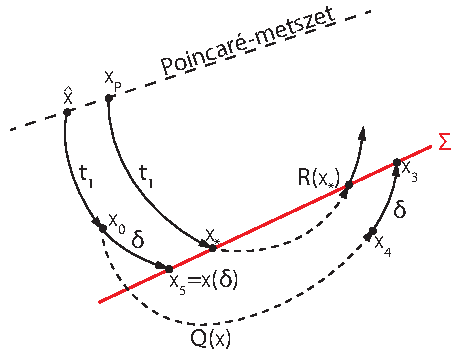
\includegraphics[width=0.5\textwidth]{graphics/korrKapcs1.png}
\caption{Periodikus pálya a kapcsolóvonal közelében.}
\end{figure}

Azaz melyik az a leképezés, amely $\hat{x}$-ból indítva $t_1$-ig (és \emph{nem} $t_1+\delta$-ig) integrálva olyan pontba visz, hogy onnan újabb $\delta$-ig integrálva a helyes $x_3$ pontba érkezünk? Másképp fogalmazva, meghatározandó az a $Q(x)$ leképezés, amely $x_0$ pont $x_4=Q(x_0)$ képéből indulva $\delta$ ideig integrálva ugyanúgy $x_3$-ba visz, mintha $x_5$ pontban alkalmaztuk volna az $R(x)$ leképezést.
\par Tehát meg kell konstruálnunk a $x_0\mapsto Q(x_0)=x_4$ leképezést.
A megoldást $x_0$ körül, kis $\delta$ értékekre sorbafejtve kapjuk, hogy:
%
\begin{equation}
x_5=x(\delta)=\Phi(x_0,\delta)|_{t=0}=x_0+\delta F(x_0)+\mathcal{O}(\delta^2).
\end{equation}
%
Legyen $x_0=x^*+\Delta x$, ezt behelyettesítve a fenti egyenletbe kapjuk, hogy
%
\begin{equation}
x(\delta)=x^*+\Delta x+\underbrace{\delta F(x^*+\Delta x)}_{ F|_{\Delta x=0}= F(x^*)+\underbrace{\Delta x \cdot \textvisiblespace\,}_{\delta \Delta x \approx 0} }+\mathcal{O}(\delta^2)=x^*+\Delta x+\delta F(x^*)+\mathcal{O}(\delta^2,\delta \, \Delta x, \Delta x^2)
\end{equation}
Másrészről, mivel $x_5=x(\delta)$ rajta van a kapcsolófelületen:
%
\begin{equation}
O=H(x(\delta))=H(x^*+\Delta x+\delta F(x^*)+\mathcal{O}(\delta^2,\delta \, \Delta x, \Delta x^2))\,,
\end{equation}
%
valamint $H(x)$ sorfejtése $x^*$ körül 
%
\begin{equation}
H(x)|_{x=x^*}=\underbrace{H(x^*)}_{=0}+H_x(x^*)(x-x^*)+\mathcal{O}(\|{x-x^*}\|^2)\,,
\end{equation}
tehát:
\begin{equation}
O=H_x(x^*)(\Delta x+\delta F(x^*))+\mathcal{O}(2)\,.
\end{equation}

Így $\delta$-ra adódik, hogy:
\begin{equation}
\delta=-\frac{H_x(x^*)\Delta x}{H_x(x^*)F(x^*)}+\mathcal{O}(2)\,,
\end{equation}
amely azt jelenti, hogy a kapcsolófelület $H_x(x)$ gradiensét kell kiértékelni $x^*$ helyen ahhoz, hogy becslést tudjunk adni a szükséges korrekcióra. A becslés hibája $\mathcal{O}(2)$, így a kapcsolófelület ferdeségét figyelembe véve becsülhető a $\delta$ idő, amely alatt a zavart $\hat x$ pontból indított megoldás $t_1$ idő elteltét követően elérte volna a kapcsolófelületet.\par
% <img src="korrKapcs2.png" width="300px"/>
Továbbá:
\begin{align}
x_3&=R(x(\delta))=R(x^*+\Delta x+\delta F(x^*)+\mathcal{O}(2))\,, \\
x_4&=\Phi(x_3,-\delta)|_{t=0}=x_3-\delta F(x_3)+\mathcal{O}(\delta^2) \,,
\end{align}
amiből az $x_4$ az $x^*$ körül:
\begin{multline}
\left.x_4\right|_{x^*}=\underbrace{R(x^*)+R_x(x^*)\overbrace{(\Delta x+\delta F(x^*))}^{-x^*+x(\delta)}}_{x_3}-\delta F\underbrace{(R\overbrace{(x^*+\Delta x+\delta F(x^*))}^{x(\delta)}}_{x_3})+\mathcal{O}(2)=\\
=R(x^*)+R_x(x^*)\Delta x+ \delta [R_x(x^*)F(x^*)-F(R(x^*))]+\mathcal{O}(2)\,.
\end{multline}

Mivel $\Delta x=x_0-x^*$ a keresett $x_0 \mapsto Q(x_0)=x_4$ leképezés, ezért 
\begin{equation}
Q(x_0)|_{x^*}=R(x^*)+R_x(x^*)\Delta x-\frac{H_x(x^*)\Delta x}{H_x(x^*)F(x^*)}(R_x(x^*)F(x^*)-F(R(x^*)))\,,
\label{linearizaltx4}
\end{equation}
%
ahol az $x_0$ aktuális helye  függ az $\hat{ x}$-tól, tehát a perturbáció mértékétől, így $\Delta x$ szintén a zavarástól függ.
 $Q_x$ leképezés szintén linearizálható $x^*$ körül, amely $x_0$ helyen: 
\begin{equation}
Q(x_0)|{x^*}=R(x^*)+Q_x(x^*)\Delta x\,.
\label{linearizaltlekepezes}
\end{equation}
%
Ebből a \ref{linearizaltlekepezes} egyenletben szereplő $Q_x(x^*)$ mátrix meghatározható $\Delta x$ együtthatóinak kigyűjtésével \ref{linearizaltx4} egyenletből:
\begin{equation}
Q_x(x^*)=R_x(x^*)+\frac{F(R(x^*))-R_x(x^*)F(x^*)}{H_x(x^*)F(x^*)}H_x(x^*)\,.
\end{equation}

\section{Példa}
Vegyük a következő folytonos rendszert:
\[F(x) = \left(
\begin{matrix}
x_2\\
-x_1 - 2 \xi x_2 + \mathrm{cos}(\omega t)\\
1
\end{matrix}
\right) = \left(
\begin{matrix}
x_2\\
a\\
1
\end{matrix}
\right),
\]
továbbá a kapcsolóvonal 
$ H(x) =  x_1 - \delta \quad$, vagyis $x_1 = \delta$-nál fal van, így
$ R(x) = \left(x_1,-rx_2,x_3\right)^\mathrm{T} \quad$, melynek $x$ szerinti deriváltja
\[R_x(x) = 
\left(
\begin{matrix}
1 & 0 & 0 \\
0 & -r & 0 \\
0 & 0 & 1
\end{matrix}
\right)\]
\textsl{(Megj.: $\delta$ a levezetések során egy időtartamot jelölt, a feladatbeli jelentése egy távolság.)}\par
A becsapódás normál sebessége: $v = H_x(x^*) F(x^*)=x_2^*$, továbbá jelölje $a^-$ és $a^+$ az ütközés előtti és utáni pillanatbeli értékeket, vagyis
$a^- = -x_{1}^* - 2 \xi x_{2}^* + \mathrm{cos}(\omega t)$ és
$a^+ = -x_{1}^* + 2 \xi r x_{2}^* + \mathrm{cos}(\omega t)$.

Ezekkel:
$ Q_x = 
\underbrace{\left(\begin{matrix}
1 & 0 & 0 \\
0 & -r & 0 \\
0 & 0 & 1
\end{matrix}\right)}_{R_x\left(x^*\right)} +
\underbrace{\frac{1}{v}}_{\frac{1}{H_x\left(x^*\right) F\left(x^*\right)}}
\left(
\underbrace{
\left(
\begin{matrix}
-rv \\
a^+ \\
1
\end{matrix}
\right)}_{F\left(R \left(x^* \right) \right)}-
\underbrace{
\left(
\begin{matrix}
1 & 0 & 0 \\
0 & -r & 0 \\
0 & 0 & 1
\end{matrix}
\right)}_{R_x\left(x^*\right)}
\underbrace{
\left(
\begin{matrix}
v \\
a^- \\
1
\end{matrix}
\right)
}_{F\left(x^*\right)}
\right)
\underbrace{
\left(
\begin{matrix}
1 & 0 & 0
\end{matrix}
\right)
}_{H_x\left(x^*\right)}
= \\
=
\left(
\begin{matrix}
1 & 0 & 0 \\
0 & -r & 0 \\
0 & 0 & 1
\end{matrix}
\right) + \frac{1}{v}
\left(
\begin{matrix}
-rv -v \\
a^+ + ra^- \\
0
\end{matrix}
\right)
\left(
\begin{matrix}
1 & 0 & 0
\end{matrix}
\right)
= \\
=
\left(
\begin{matrix}
1 & 0 & 0 \\
0 & -r & 0 \\
0 & 0 & 1
\end{matrix}
\right) + \frac{1}{v}
\left(
\begin{matrix}
-rv -v & 0 & 0\\
a^+ + ra^- & 0 & 0\\
0 & 0 & 0
\end{matrix}
\right)
=
\left(
\begin{matrix}
-r & 0 & 0\\
\frac{a^+ + ra^-}{v} & -r & 0\\
0 & 0 & 1
\end{matrix}
\right)
$\linebreak
\textsl{(Megj.: A skalár gradiensét (pl. most: $H_x(x))$ sorvektorként értelmezzük, ami egybevág azzal, hogy a Jacobi mátrix sorai is a vektor adott elemének mint skalárnak a gradiensét tartalmazzák)}


\section{Transzverzális metszés, általános eset}

%Itt sokminden le van gépelve, csak ki van kommentelve.

Korrekció a kapcsolósíkon. Az általános esetben:
\[
{\dot{x}} = \begin{cases}
   {\ F}_1(x), & \text{ha } \; H({ x})>0 \\
   {\ F}_2(x), & \text{ha } \; H({ x})<0, 
 \end{cases}
\]


%\begin{wrapfigure}{r}{5cm}
\begin{figure}
	\centering
	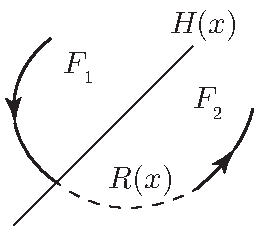
\includegraphics[width=0.35\textwidth]{graphics/5_1.png}
	\caption{$R(x)$ nem kapcsolósíkra képez le.}\label{fig:501}
\end{figure} 
%\end{wrapfigure} 


ahol ${x}\rightarrow R({x}),\; \text{ha}\; H(x)=0.$ Továbbá $R(x)$-nek nem kötelező a kapcsolósíkra leképeznie (lásd \ref{fig:501}. ábra).\\

 A $Q(x)$ korrekciós leképezés alatt a következő érthető: (lásd \ref{fig:502}. ábra)
\noindent
 $\Sigma = \lbrace x,\; H(x)=0 \rbrace,\\
 x^*=\Phi_1(x_p,t),\\
 x_0=\Phi_1{(\hat{x},t_1)} \rightarrow x_2=\Phi_1(x_0,\delta),\\
 x_4=\Phi_2(x_3,-\delta),\\
 x_0 \rightarrow x_4=Q(x_0)=\Phi_2(\underbrace{R(\overbrace{\Phi_1(x_0,\delta)}^{x_2})}_{x_3},-\delta)$

\begin{figure}[ht]
\centering
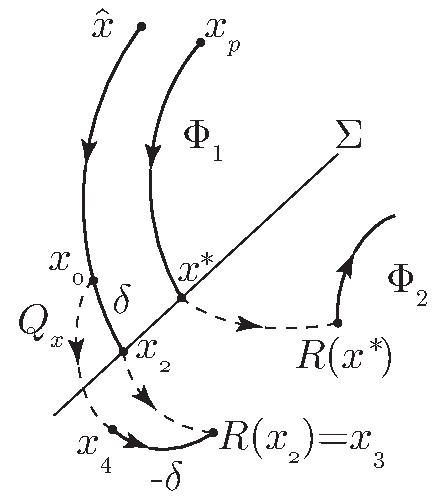
\includegraphics[width=0.4\textwidth]{graphics/5_2.png}
\caption{Korrekció származtatása ha $R(x)$ nem kapcsolósíkra képez le.}\label{fig:502}
\end{figure}

 $Q(x)$ linearizáltjára adódik, hogy:
 \begin{equation}
  Q_x(x^*)=R_x(x^*)+\frac{(F_2(R(x^*))-R_x(x^*)F_1(x^*))H_x(x^*)}{H_x(x^*)F_1(x^*)}
 \end{equation}
  és $H_x(x^*)F_1(x^*)\neq 0$ transzverzális metszés.



 \textbf{Példa 1.)} Filippov rendszer csúszás nélkül, azaz $F_1|_\Sigma \neq F_2|_\Sigma$, valamint $R(x)=x$, azaz önmagába leképezés. \\
 Ilyenkor:
 \[Q_x=I+\frac{(F_2-F_1)H_x}{H_xF_1}, \; \text{mert} \; R(x)=I.\]

 \textbf{Példa 2.)} Ütközéses dinamikai rendszer, ahol $F_1=F_2=F$.
Így $Q(x):$
\[
Q_x(x^*)=R_x(x^*)+\frac{(F(R(x^*))-R_x(x^*)F(x^*))H_x(x^*)}{H_x(x^*)F(x^*)}
\]

 \textbf{Példa 3.)} Filippov rendszer csúszással, azaz
 
 \[
 F_s=F_{12}=(1-\alpha)F_1+\alpha F_2, \; \text{és } \; \alpha=\frac{H_x F_1}{H_x(F_1-F_2)}.
 \]
 Ekkor
\[
	Q_x=F+\frac{(F_{12}-F1)H_x}{H_xF_1}
\]

\begin{figure}[ht]
	\centering
	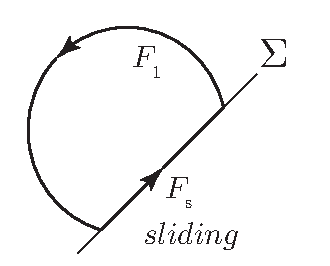
\includegraphics[width=0.4\textwidth]{graphics/5_3.png}
	\caption{Filippov rendszer csúszással}\label{fig:503}
\end{figure}
\clearpage


\input{korrekcio_a_kapcsolofeluleten2}
\chapter{\label{sec:perpalyakovetes}Periodikus pályák numerikus követése}

Dinamikai rendszerek vizsgálatánál kíváncsiak vagyunk a rendszer viselkedésére különböző paraméterkombinációk esetében is.
A paraméterek ha\-tá\-sá\-nak vizsgálatára többféle módszer is rendelkezésünkre áll, mint például a paraméterléptetés vagy a pszeudo-ívhossz módszer.
Paraméterléptetés esetén a bifurkációs paraméter értékét kis mértékben megváltoztatjuk, ekkor jól megfogalmazott probléma esetén a megoldás is kis mértékben fog változni, és ezt a változást követjük lépésről-lépésre.
Pszeudo-ívhossz mód\-szer\-nél a bifurkációs paraméter és a periódikus pálya periódusidejének össze\-füg\-gé\-sét keressük oly módon, hogy a problémát egy "szintvonal" keresésre vezetjük vissza.
A fejezetben ez utóbbival fogunk részletesebben foglalkozni.

\section{Pszeudo-ívhossz módszer}
\label{sec:pseudo_ivhossz}

A pszeudo-ívhossz módszer esetében a soron következő megoldást az előző megoldástól $\mathbf{v}$ irányba keressük, ahol $\mathbf{v}$ egy implicit egyenlet $F(\mathbf{x}) = 0$ szintvonalának érintőjével párhuzamos egységhosszú vektor:
\begin{equation}
\begin{cases}
0 = \left< \mathbf{x}_{i+1} - \mathbf{x}_i, \mathbf{v}_i \right> - \Delta s \\
0 = F(\mathbf{x}_{i+1}),
\end{cases}
\label{eq:pszeudo_ivhossz_alapegyenlet}
\end{equation}
\begin{equation}
\mathbf{x_i}= \begin{bmatrix}
x_i & y_i
\end{bmatrix}^\mathrm{T},
\end{equation}
és $\Delta s$ a lépés ívhossza.
Az első egyenlet a merőlegességi feltétel, a második magának a keresett szintvonalnak az egyenlete.
A módszer egy iterációs lépésének szemléltetése a \ref{fig:pszeudo_ivhossz_szemleltet}. ábrán látható.
A merőlegességi feltétel az alábbi módon vezethető le:
\begin{equation}
\hat{\mathbf{x}} = \mathbf{x}_i + \Delta s \, \mathbf{v}_i,
\end{equation}
\begin{equation}
\begin{matrix}
\left< \mathbf{x}_{i+1} - \hat{\mathbf{x}}, \mathbf{v}_i \right> & = & 
\left< \mathbf{x}_{i+1} - \mathbf{x}_i - \Delta s \, \mathbf{v}_i, \mathbf{v}_i \right>  & = \\
\left< \mathbf{x}_{i+1} - \mathbf{x}_i, \mathbf{v}_i \right> - \Delta s \, \left< \mathbf{v}_i , \mathbf{v}_i \right> & = & \left< \mathbf{x}_{i+1} - \mathbf{x}_i, \mathbf{v}_i \right> - \Delta s. & \blacksquare 
\end{matrix}
\end{equation}

\begin{figure}[ht]
	\centering
	\includegraphics[width=0.4\textwidth]{graphics/pszeudo_ivhossz_szemleltet.png}
	\caption{A pszeudo-ívhossz módszer egy iterációs lépésének szemléltetése}\label{fig:pszeudo_ivhossz_szemleltet}
\end{figure}

A módszer alkalmazása során a \eqref{eq:pszeudo_ivhossz_alapegyenlet} egyenletrendszert szimultán kell megoldani $\mathbf{x}_{i+1}$-re - két egyenlet, két ismeretlen.
A módszer általánosítható több dimenzióra is, ekkor több $F_j(\mathbf{x})$ egyenletre van szük\-sé\-günk.

Egy \textbf{példa} a módszer alkalmazására az egység sugarú kör körívének követése.
Akkor az implicit függvényünk az alábbi:
\begin{equation}
F(\mathbf{x}) = x^2 + y^2 -1.
\end{equation}
A kezdőpontunk legyen
\begin{equation}
\mathbf{x}_0 = \begin{bmatrix}
1 & 0
\end{bmatrix}^\mathrm{T},
\end{equation}
amely, mint látható kielégíti az implicit egyenletünket.
A sebességvektor, azaz az érintő ebben a pontban
\begin{equation}
\mathbf{v}_0 = \begin{bmatrix}
0 & 1
\end{bmatrix}^\mathrm{T}.
\end{equation}
Azonban az esetek többségében ez nem ilyen egyszerűen meghatározható, és numerikusan kell közelítenünk, amihez ismernünk kell a szintvonal egy másik, közeli pontját is, $\mathbf{x}_{1/2}$-et:
\begin{equation}
\mathbf{v}_0 = \frac{\mathbf{x}_{1/2} - \mathbf{x}_{0}}{\left \| \mathbf{x}_{1/2} - \mathbf{x}_{0} \right \|}.
\end{equation}
A sebességvektor ezek után rendre:
\begin{equation}
\mathbf{v}_i = \frac{\mathbf{x}_{i} - \mathbf{x}_{i-1}}{\left \| \mathbf{x}_{i} - \mathbf{x}_{i-1} \right \|}.
\end{equation}
A körív követésének eredménye a pszeudo-ívhossz módszerrel a \ref{fig:pszeudo_ivhossz_koriv}. ábrán látható.
A lépéshossz $\Delta s = 0.1$ volt, a kezdeti sebességbecsléshez az $\mathbf{x}_0$-hoz közeli szintvonal pont pedig
\begin{equation}
\mathbf{x}_{1/2} = \begin{bmatrix}
0.99 & \sqrt{1 - 0.99^2}
\end{bmatrix}^\mathrm{T}.
\end{equation}

\begin{figure}[ht]
	\centering
	\includegraphics[width=0.8\textwidth]{graphics/pszeudo_ivhossz_koriv}
	\caption{A pszeudo-ívhossz módszer alkalmazása körív követésére}\label{fig:pszeudo_ivhossz_koriv}
\end{figure}

\textbf{Megjegyzés:} pontosabb sebességvektort kapunk az iteráció során, ha a megoldáskor $\mathbf{x}_{i+1/2}$-re is alkalmazzuk a pszeudo-ívhossz módszert, ekkor a sebességvektor általánosan így írható fel:
\begin{equation}
\mathbf{v}_i = \frac{\mathbf{x}_{i+1/2} - \mathbf{x}_{i}}{\left \| \mathbf{x}_{i+1/2} - \mathbf{x}_{i} \right \|}.
\end{equation}
Az így keletkező extra egyenletek ugyanolyan formájúak, mint a \eqref{eq:pszeudo_ivhossz_alapegyenlet} egyenlet az alábbi indexelést alkalmazva a problémára:
\begin{equation}
\begin{cases}
0 = \left< \mathbf{x}_{i+3/2} - \mathbf{x}_{i+1/2}, \mathbf{v}_i \right> - \Delta s \\
0 = F(\mathbf{x}_{i+3/2}),
\end{cases}
\end{equation}
Összességében ez a feladat egy négyváltozós nemlineáris gyökkeresési probléma az eredeti kétváltozós helyett.

\section{Periodikus pályák peremérték-megfogalmazása}
\label{sec:per_palya_perem_megfog}

Dinamikai rendszerek mozgásegyenleteinek megoldásakor kezdeti értéket szoktunk megadni.
Amennyiben a rendszer periódikus mozgást végez, a probléma átírható egy peremérték feladatra, ahol a peremfeltételt a periódus elejére és végére kell előírni.
Belátható ugyanis, hogy periódikus mozgásnál az állapotváltozóknak $t_0$ és $t_0 + T$ időpontokban meg kell egyezniük, ahol $T$ a periódusidő.
Dinamikai rendszerek mozgásegyenleteit Cauchy átírással általánosan az alábbi módon lehet megadni:
\begin{equation}
\dot{\mathbf{z}}(t) = \mathbf{F}(\mathbf{z}(t)),
\label{eq:EOM_altalanosan}
\end{equation}
ahol $\mathbf{z}(t)$ az állapotváltozók, $\mathbf{q}(t)$ pedig az általános koordináták vektora:
\begin{equation}
\mathbf{z}(t) = \begin{bmatrix}
\mathbf{q}(t) & \dot{\mathbf{q}}(t)
\end{bmatrix}^\mathrm{T}.
\end{equation}
Periódikus mozgás esetén (autonóm rendszereknél $t_0$ szabadon megválasztható, így vegyük zérusnak) igaz a következő
\begin{equation}
\mathbf{z}_\mathrm{p}(0) = \mathbf{z}_\mathrm{p}(T) .
\end{equation}

Vezessük be $\tau$ dimenziótlan időt az alábbi módon:
\begin{equation}
\tau =  t/T.
\end{equation}
Ekkor a \eqref{eq:EOM_altalanosan} egyenlet formája és a peremérték feladat a következő lesz
\begin{equation}
\begin{cases}
\mathbf{z}'(\tau) = T\,\mathbf{F}(\mathbf{z}(\tau)), \\
\mathbf{z}(0) = \mathbf{z}(1).
\end{cases}
\label{eq:EOM_dimtalan}
\end{equation}

\textbf{Megjegyzés:} amennyiben a rendszerünk szakaszosan folytonos a \eqref{eq:EOM_dimtalan}-es problémát ki kell egészíteni:
\begin{equation}
\begin{matrix}
\begin{cases}
\mathbf{z}'(\tau_1) = T_1\,\mathbf{F}_1(\mathbf{z}(\tau_1)), \; H(\mathbf{z}(\tau_1)) > 0,\\
\mathbf{z}'(\tau_2) = T_2\,\mathbf{F}_2(\mathbf{z}(\tau_2)), \; H(\mathbf{z}(\tau_2)) < 0,
\end{cases} \\\\
\begin{cases}
\mathbf{z}_1(1) = \mathbf{z}_2(0), \\
\mathbf{z}_2(1) = \mathbf{z}_1(0),
\end{cases} \\\\
\begin{cases}
H(\mathbf{z}_1(1)) = 0, \\
H(\mathbf{z}_2(1)) = 0,
\end{cases}
\end{matrix}
%\label{eq:EOM_dimtalan}
\end{equation}
ahol $H(\mathbf{z}(\tau))$  a kapcsolófelület.
Ütköző rendszer esetében figyelembe kell venni a peremfeltételek felírásánál az ütközéskor létrejövő leképezést.

Nézzük meg egy egyszerű \textbf{példa} peremérték-megfogalmazásának implementálását MATLAB környezetben!
Peremérték feladatok megoldására a bvp beépített megoldókat lehet használni, esetünkben a bvp5c-vel fogunk dolgozni.
A mechanikai rendszerünk a \ref{fig:bvp_tomeg_rugo}. ábrán látható.

\begin{figure}[ht]
	\centering
	\includegraphics[width=0.3\textwidth]{graphics/tomeg_rugo_modell}
	\caption{Periódikus mozgást végző tömeg-rugó rendszer}\label{fig:bvp_tomeg_rugo}
\end{figure}

A mozgásegyenlete a fenti rendszernek jól ismert:
\begin{equation}
\ddot{x}= -\frac{k}{m}\,x.
\end{equation}
Mint tudjuk, a rendszer mozgását leíró függvényt az alábbi módon lehet felírni, amennyiben $x_0$ kezdeti kitérítésünk van csak $\tau_0$ időpillanatban kezdeti sebesség nélkül:
\begin{equation}
\varphi(\tau) = x_0\cos\left(\tau\sqrt{k/m}\,T\right) = x_0\cos\left(2\pi\,\tau\right),
\end{equation}
\begin{equation}
\dot{\varphi}(\tau) = -x_0\sqrt{k/m}\sin\left(\tau\sqrt{k/m}\,T\right) = -x_0\sqrt{k/m}\sin\left(2\pi\,\tau\right),
\end{equation}
ahol $T$ a rendszer sajátfrekvenciájának inverze
\begin{equation}
T = 2\pi\sqrt{m/k}.
\end{equation}
A fenti függvényeket a peremérték-megfogalmazáskor kijöttekkel fogjuk összevetni.

A bvp5c megoldóhoz először definiálnunk kell egy időrácsot, amely i\-dő\-pon\-tok\-ban meg kell becsülnünk majd a keresett függvények értékét.
Mivel áttértünk dimenziótlan időre, egy periódus "peremei" a $\tau \in \left \{ 0,1 \right \}$ pontok, valamint megjelent a Cauchy átírásnál $T$ periódusidő, mint ismeretlen paraméter.
\begin{equation}
\begin{bmatrix}
x'(\tau) \\ y'(\tau)
\end{bmatrix} = 
T
\begin{bmatrix}
y(\tau) \\  -\frac{k}{m}\,x(\tau)
\end{bmatrix} 
\end{equation}
A módszer a rácsháló első és utolsó pontjára fogja alkalmazni a peremfeltételeket.
Jó kezdeti függvénybecslés a megoldó megfelelő működéséhez az egyik legfontosabb kritérium, ehhez minél több információt össze kell gyűjteni a vizsgált rendszer viselkedéséről.
A kezdeti függvénybecslésnek teljesítenie kell a peremfeltételeket.%, melyeknek rajta kell lenniük a periódikus pályán.
Az ismeretlen paraméter(ek)re is szükséges kezdeti becslést adni!
A peremfeltételeket megadó vektor (res $\in \mathbb{R}^r = \mathbb{R}^{n+p}$) dimenziója megegyezik a mozgásegyenlet (dydx $\in \mathbb{R}^n$) és a paramétereket tartalmazó vektor (par $\in \mathbb{R}^p$) dimenziójának összegével.
\begin{lstlisting}
global k m x0
k = 10;
m = 5;
x0 = 1;
taumesh = linspace(0,1,5);
par = 2*pi;
solinit = bvpinit(taumesh, @bvp_initial_guess, par);
sol = bvp5c(@bvp_fun, @bvp_bcs, solinit);

function g = bvp_initial_guess(x)
global x0
g = x0*[cos(2*pi*x); -2*pi*sin(2*pi*x)];
end

function dydx = bvp_fun(x,y,par)
global k m
dydx = par*[y(2); -k*y(1)/m];
end

function res = bvp_bcs(ya,yb,par)
global x0
res = [ya(1) - x0
    yb(1) - x0
    ya(2)];
end
\end{lstlisting}

A módszer által kiszámolt $T$ értéke megegyezik az analitikusan kiszámított periódusidővel.
A tömegpont pozíciója és sebessége a \ref{fig:bvp_tomeg_rugo_traj_vel}. ábrán látható.

\begin{figure}[ht]
	\centering
	\includegraphics[width=0.75\textwidth]{graphics/BVP_tomeg_rugo}
	\caption{Tömeg-rugó rendszer peremérték-megfogalmazásának bvp5c megoldóval kiszámított eredményeinek összevetése az analitikus megoldással}\label{fig:bvp_tomeg_rugo_traj_vel}
\end{figure}

\section{Pszeudo-ívhossz módszer alkalmazása periodikus pályák kö\-ve\-té\-sé\-hez}

Ebben az alfejezetben két példát nézünk meg, ahol a pszeudo-ívhossz mód\-szert periódikus pályák követésére használjuk.
Ehhez ki kell választanunk majd egy bifurkációs paramétert, amely függvényében kíváncsiak vagyunk, hogyan alakul a periódikus mozgás.
Az első feladat során az előbb vizsgált tömeg-rugó rendszerrel foglalkozunk, a másodikban egy szakaszosan folytonos rendszert, a spring loaded inverted pendulom (SLIP) modellt vizsgáljuk, amely az emberi futás leírásának egy elterjedten használt modellje.

\subsection{Példa 1: tömeg-rugó rendszer}

A pszeudo-ívhossz módszer használatához ki kell választanunk egy bi\-fur\-ká\-ci\-ós paramétert, amit jelöljön $\mu$.
A példa során először vizsgáljuk a rugómerevség $(\mu = k)$, később a tömeg $(\mu =m)$ hatását (ilyenkor a többi paraméter konstans).
A \eqref{eq:pszeudo_ivhossz_alapegyenlet} egyenlet alakja paraméterkövetés során az alábbi formájú:
\begin{equation}
\begin{cases}
0 = \left< \mathbf{x}_{i+1} - \mathbf{x}_i, \mathbf{v}_i \right> - \Delta s \\
0 = T_{i+1} - T_{\mathrm{BVP}}(\mu_{i+1}),
\end{cases}
\label{eq:pszeudo_per_kov}
\end{equation}
\begin{equation}
\mathbf{x_i}= \begin{bmatrix}
\mu_{i} & T_{i}
\end{bmatrix}^\mathrm{T},
\end{equation}
ahol $T_{\mathrm{BVP}}(\mu_{i+1})$ a peremfeladat megoldó által számolt periódusidő.
A psze\-u\-do-ív\-hossz módszert a \ref{sec:pseudo_ivhossz} alfejezetben bemutatott módon kell alkalmazni, és a benne található $T_{\mathrm{BVP}}(\mu_{i+1})$ értékét a \ref{sec:per_palya_perem_megfog} alfejezetben leírt módon kell meghatározni a \eqref{eq:pszeudo_per_kov} egyenletrendszer megoldása közben.
A kapott eredményeket összevetettük az analitikusan kiszámítottakkal, és látható, hogy a pályakövetés illeszkedik az analitikusan előállított görbékre, ld. \ref{fig:pszeudo_tomeg_rugo_k}. és \ref{fig:pszeudo_tomeg_rugo_m}. ábrák.

\begin{figure}[ht]
	\centering
	\includegraphics[width=0.9\textwidth]{graphics/pszeudo_tomeg_rugo_k}
	\caption{Periódikus pályák követése $k$ paraméter függvényében, $\Delta s = 0.5$}\label{fig:pszeudo_tomeg_rugo_k}
\end{figure}

\begin{figure}[ht]
	\centering
	\includegraphics[width=0.9\textwidth]{graphics/pszeudo_tomeg_rugo_m}
	\caption{Periódikus pályák követése $m$ paraméter függvényében, $\Delta s = 1$}\label{fig:pszeudo_tomeg_rugo_m}
\end{figure}

\subsection{Példa 2: spring loaded inverted pendulom modell}

A spring loaded inverted pendulum (SLIP) modell a \ref{fig:SLIP_mechanikai_modell}. ábrán látható.
A rendszer egy tömegpontból és egy tömeg nélküli rugóból áll, ami $\alpha$ szögben kapcsolódik a tömegponthoz.
A SLIP modell az emberi futás modellezéséhez használt egyszerű mechanikai modell.
Periódikus mozgásra képes, mely mozgás két fázisra, a támasz és repülő fázisokra tagolódik, így a rendszer szakaszosan, de $\mathrm{C}^2$ folytonos.

\begin{figure}[ht]
	\centering
	\includegraphics[width=0.9\textwidth]{graphics/slip_mozgas}
	\caption{Spring loaded inverted pendulum (SLIP) mechanikai modellje}\label{fig:SLIP_mechanikai_modell}
\end{figure}

A rendszer mozgásegyenlete a támaszfázisban (mivel az $x$ kvázi ciklikus koordináta (a kezdeti értéke nem befolyásolja a mozgás minőségét, amennyiben a repülőfázisból vagy fá\-zis\-ha\-tá\-rok\-ról indítjuk a rendszert), a rugó megfogott végét önkényesen mindig az origóba helyezzük, ami a tömegpont $x$ koordináta szerinti helyzetét is megadja a fázis elején), és az állapotváltozók az alábbiak:
\begin{equation}
\begin{cases}
\ddot{x} = \kappa\left(l_0 - l(t) \right)x(t)/l(t),\\
\ddot{y} = \kappa\left(l_0 - l(t) \right)y(t)/l(t) - g,
\end{cases}
\end{equation}
\begin{equation}
\mathbf{z}(t)= \begin{bmatrix}
x(t) & y(t) & \dot{x}(t) & \dot{y}(t)
\end{bmatrix}^\mathrm{T},
\end{equation}
\begin{equation}
l(t) = \sqrt{\left(-x(t)\right)^2 + y(t)^2},
\end{equation}
A repülő fázisban is a fenti mozgásegyenlet érvényes, csupán a $\kappa = s/m = 0$ helyettesítést kell alkalmazni.
A fázishatárokat megadó eseményfüggvények a támasz-repülő fázishatáron, illetve a repülő-támasz fázishatáron az a\-láb\-bi\-ak, ahol az 1-es index a támaszfázis, a 2-es a repülőre vonatkozik:
\begin{equation}
\begin{matrix}
H_{12}(\mathbf{z}) = l_0 - l(t), \\
H_{21}(\mathbf{z}) = y(t) - l_0\cos(\alpha).
\end{matrix}
\end{equation}

A peremfeladat megoldásához a mozgásegyenletekre alkalmazni kell a Cauchy-átírást, illetve dimenziótlanítani kell idő szerint.
Külön kell dimenziótlanítani a támaszfázis mozgásegyenleteit a $\tau_1 = t/T_1$ dimenziótlan idővel felírva, és külön a repülőfázisét $\tau_2 = t/T_2$-vel.
\begin{equation}
\begin{matrix}
\begin{cases}
\mathbf{z}'(\tau_1) = T_1\,\mathbf{F}_1(\mathbf{z}(\tau_1)), \; H_{12}(\mathbf{z}(\tau_1)) > 0, \\
\mathbf{z}'(\tau_2) = T_2\,\mathbf{F}_2(\mathbf{z}(\tau_2)), \; H_{21}(\mathbf{z}(\tau_2)) > 0,
\end{cases} \\\\
\begin{cases}
\mathbf{z}_1(1) = \mathbf{z}_2(0), \\
\hat{\mathbf{z}}_2(1) = \hat{\mathbf{z}}_1(0),
\end{cases} \\\\
H_{12}(\mathbf{z}_1(1)) = 0,
 \\\\
x_1(0) = -l_0\sin{\alpha},
\\\\
\hat{E} = l_0\cos(\alpha)\,g + \left(x'_2(1)^2 + y'_2(1)^2\right)/2,
\end{matrix}
\end{equation}
ahol
\begin{equation}
	\hat{\mathbf{z}}(\tau) = 
	\begin{bmatrix}
		y(\tau) & x'(\tau) & y'(\tau)
	\end{bmatrix}^\mathrm{T},
\end{equation}
ugyanis $x(\tau)$ kvázi ciklikus koordináta, melynek értéke periódikus mozgás során szigorú monoton nő, így $\mathbf{z}_1(0)\neq\mathbf{z}_2(1)$, viszont $x_1(0)$ ismert.
Valamint $\hat{E}$ a tömeg szerint fajlagosított mechanikai összenergia, amely a rendszer egy paramétere, hiszen a modell konzervatív.
A $H_{21}(\mathbf{z}_2(1))$ helyett azért jobb a fenti egyenlet használata, mivel ez a kapcsolófelület által tartalmazott információn felül többet mondd, és kijelöli, hogy milyen energiaszinten mozog a rendszer.
A \eqref{eq:pszeudo_per_kov} egyenletben a $T_{\mathrm{BVP}}(\mu_{i+1}) = T_{\mathrm{BVP,1}}(\mu_{i+1}) + T_{\mathrm{BVP,2}}(\mu_{i+1})$ helyettesítést kell alkalmazni a peremfeladat megoldása után.

Egy jó próbafüggvény megadásához először inicializáljuk a feladatot, azaz keresünk egy periódikus pályát.
A feladatot a támaszfázis elejéről indítjuk, és itt $y_1(0) = l_0\cos(\alpha)$ ismert, valamint $x(\tau)$ kvázi ciklikus koordináta.
Mivel a rendszer konzervatív a mechanikai összenergiát paraméternek választva a sebességkomponensek kifejezhetők egymásból a támaszfázis elején, mi a $\dot{x}_1(0)$-t vesszük most független változónak.
A rendszer mozgását tehát adott paraméterkombinációnál egy változó fogja befolyásolni a támaszfázis bal oldali peremén.
Az inicializálásnál az alábbi egyenlet zérushelyét keressük meg:
\begin{equation}
	f(\dot{x}_1(0)) = \dot{x}_1(0) - \dot{x}_2(1) = 0.
\end{equation}
Az inicializált kezdeti próbafüggvényekben a periódikus pálya pontjait hasz\-nál\-juk fel, ahol az időpillanatokat az $xini$, a függvényértékeket az $yini$ változókba mentjük.
Az inicializált kezdeti próbafüggvények a $\dot{x}_1(0) = 5.1149\; \mathrm{m/s}$ kezdeti értékű pe\-ri\-ó\-di\-kus pályához vannak felírva, ahol a paraméterek értéke $l_0 = 1 \; \mathrm{m}$, $\kappa = 112.5\;\mathrm{N/(m\,kg)}$, $\alpha = 0.5708 \;\mathrm{rad}$, $\hat{E} = 21.5 \;\mathrm{N/kg}$.
A pszeudo-ívhossz iterációjában az $xini$ és $yini$ változókat mindig aktualizáljuk a peremfeladat megoldó által számított megoldással.
Fel\-té\-te\-lez\-zük, hogy a változás a pálya képében folyamatos a paraméterek változásával. 
A MATLAB kód lényeges részei lentebb megtekinthetők.
\begin{lstlisting}
for i = 1:imax	
xi_p = start_pseudo_root_finding();	
v = (xi_p-xi)/norm((xi_p-xi));	
xi = xi_p;
end
\end{lstlisting}
\begin{lstlisting}
function y = start_pseudo_root_finding()
mu = xi(1);	
fun_PAM = @pseudo_root_finding;
x = fzero(fun_PAM,mu);	
T_par1 = T_BVP(1);
T_par2 = T_BVP(2);
[T_BVP_1,T_BVP_2]=boundary_SLIP(T_par1,T_par2);
T_BVP=[T_BVP_1,T_BVP_2,T_BVP_1+T_BVP_2];	
y = [x; T_BVP(3)];
end
\end{lstlisting}

\begin{lstlisting}
function y = pseudo_root_finding(mu)
T_par1 = T_BVP(1);
T_par2 = T_BVP(2);
[T_BVP_1, T_BVP_2]  = boundary_SLIP(T_par1, T_par2);
T_BVP = [T_BVP_1, T_BVP_2, T_BVP_1 + T_BVP_2];	
a = v(1);
b = v(2);
c = xi(1);
d = xi(2);	
T_i = (h - (mu - c)*a)/b + d;	
y = T_i - T_BVP(3);
end
\end{lstlisting}
\begin{lstlisting}
function [T1, T2] = boundary_SLIP(T_in1, T_in2)
global xdot10
global xini yini	
xinit = xini;
par = [T_in1; T_in2];
solinit = bvpinit(xinit, @bvp_initial_guess, par);
sol = bvp5c(@bvp_fun, @bvp_bcs, solinit);
T1 = sol.parameters(1);
T2 = sol.parameters(2);
xini = sol.x;
yini = sol.y;
xdot10 = sol.y(3,1);
end

function G = bvp_initial_guess(t)
global xini yini
G = [interp1(xini,yini(1,:),t)
interp1(xini,yini(2,:),t,`spline`)
interp1(xini,yini(3,:),t,`spline`)
interp1(xini,yini(4,:),t,`spline`)
interp1(xini,yini(5,:),t)
interp1(xini,yini(6,:),t,`spline`)
interp1(xini,yini(7,:),t)
interp1(xini,yini(8,:),t)];
end

function dydx = bvp_fun(t,Y,par)
global kappa_f g l0
lambda = sqrt((-Y(1))^2 + (Y(2))^2)/l0;
dydx = [par(1)*Y(3) 
par(1)*Y(4)
par(1)*( (kappa_f/lambda - kappa_f)*Y(1) )
par(1)*( (kappa_f/lambda - kappa_f)*Y(2) - g )
par(2)*Y(7)
par(2)*Y(8)
par(2)*0
-par(2)*g];
end

function res = bvp_bcs(ya,yb,par)
global l0 alpha_f 
global E_f g
res = [ya(1) + l0*sin(alpha_f)
ya(2) - yb(6)
ya(3) - yb(7)
ya(4) - yb(8)
ya(5) - yb(1)
ya(6) - yb(2)
ya(7) - yb(3)
ya(8) - yb(4)
l0 - sqrt((yb(1))^2 + (yb(2))^2) 
E_f - l0*cos(alpha_f)*g - (ya(3)^2 + ya(4)^2)/2];
end

\end{lstlisting}

A rendszer paraméterei a $\kappa$, $\alpha$, $l_0$ és $\hat{E}$, melyek közül tekintsük az $l_0$-t fixen egységnyinek.
A másik három paramétert egyenként fogjuk bifurkációs paraméterként kezelni.
A pszeudo-ívhossz módszer által megvalósított pályakövetés eredményei a \ref{fig:pszeudo_SLIP_E}., \ref{fig:pszeudo_SLIP_kappa}. és \ref{fig:pszeudo_SLIP_alpha}. ábrákon láthatók.

\begin{figure}[ht]
	\centering
	\includegraphics[width=0.8\textwidth]{graphics/pszeudo_SLIP_E}
	\caption{Pszeudó-ívhossz módszer pályakövetése, $\mu = \hat{E}$}\label{fig:pszeudo_SLIP_E}
\end{figure}

\begin{figure}[ht]
	\centering
	\includegraphics[width=0.8\textwidth]{graphics/pszeudo_SLIP_kappa}
	\caption{Pszeudó-ívhossz módszer pályakövetése, $\mu = \kappa$}\label{fig:pszeudo_SLIP_kappa}
\end{figure}

\begin{figure}[ht]
	\centering
	\includegraphics[width=0.8\textwidth]{graphics/pszeudo_SLIP_alpha}
	\caption{Pszeudó-ívhossz módszer pályakövetése, $\mu = \alpha$}\label{fig:pszeudo_SLIP_alpha}
\end{figure}

\textbf{Megjegyzés:} A \eqref{eq:pszeudo_per_kov} egyenletrendszer kipótolható egy harmadik egyenlettel, ami vonatkozhat a monodrómia mátrix sajátértékére; például kereshetjük azt a görbét, ami a stabilitáshatárt mondja meg, azaz amikor a nem triviális sajátérték $\lambda = 1$. Ekkor a mechanikai összeenergia már nem tekinthető paraméternek.
\begin{equation}
\begin{cases}
0 = \left< \mathbf{x}_{i+1} - \mathbf{x}_i, \mathbf{v}_i \right> - \Delta s, \\
0 = T_{i+1} - T_{\mathrm{BVP}}(\mu_{i+1}), \\
0 = 1 - \lambda,
\end{cases}
\end{equation}
\begin{equation}
\mathbf{x_i}= \begin{bmatrix}
\mu_{i} & T_{i} & \lambda_i
\end{bmatrix}^\mathrm{T},
\end{equation}

\chapter{\label{sec:square_root}Square-root leképezés}


Tekintsük az alábbi rendszert:
\begin{equation}
\dot{x}=F(x), \quad \text{ahol } x\in S^+=\left\{x\in\mathcal{D}\subset\mathbb{R}^n: H(x)>0\right\},
\end{equation}
amely a 
\begin{equation}
\sum:=\left\{x\in\mathcal{D}: H(x)=0\right\}
\end{equation}
felületen ütközik az
\begin{equation}
x^+=R(x^-):=x^-+W(x^-)v(x^-)
\end{equation}
leképezés által kijelölt módon. $H(x)$ a kapcsolóvonal egyenlete, $x^+$ az ütközés utáni állapotváltozó, $x^-$ pedig az ütközés előtti állapotváltozó. Az ütközés pillanatában a kapcsolófelületre merőleges sebességet és gyorsulást a 
\begin{equation}
v(x)=H_xF(x), 
\end{equation} 
a gyorsulást pedig 
\begin{equation}
 a(x)=(H_{xx}+H_xF_x)F(x)
\end{equation} 
összefüggés segítségével számíthatók ki.

\section{1DoF impakt oszcillátor}


Az 1 DoF impakt oszcillátor dimenziótlan egyenlete az alábbi:
\begin{equation}
u''(t)+2\zeta u'(t)+u(t)=w(t),\qquad u(t)>\sigma,\qquad \zeta>0.
\end{equation}
A $t=t_0$ (ütközéskori) időpillanatban az alábbi leképezés valósul meg:
\begin{equation}
f(u^-,v^-):=(u^+,v^+),
\end{equation}
ahol közvetlenül az ütközés előtti pozíció és sebesség
\begin{equation}
u^-=u(t_0),
\end{equation}
\begin{equation}
v^-=v(t_0)=\left.\frac{\mathrm{d}u}{\mathrm{d}t}\right|_{t=t_0},
\end{equation}
továbbá a közvetlenül az ütközés utáni pozíció és sebesség felírható az alábbi módon:
\begin{equation}
u^+=u^-,
\end{equation}
\begin{equation}
v^+=-rv^-, \quad 0\le r\le 1.
\end{equation}
Megjegyzés: $1-r^2$ meghatározza az ütközés során elnyelt mozgási energiaarányt. $r$ a különböző anyagok tulajdonságaitól függ, $r=0.95$ az acélrúd esetének felel meg, $r=1$ a tökéletesen rugalmas és $r=0$ a tökéletesen rugalmatlan ütközésnek felel meg. Az általunk vizsgált esetben $w(t)=\cos(\omega t)$ a periodikus gerjesztés $\frac{2\pi}{\omega}$ periódussal:
\begin{equation}
u''(t)+2\zeta u'(t)+u(t)=\cos(\omega t),\qquad u>\sigma.
\end{equation}
Az 1DoF impakt oszcillátor átírható az alábbi három-dimenziós autonóm rendszerré:
\begin{equation}
\begin{split}
\frac{\mathrm{d}u}{\mathrm{d}t}&=v,\\
\frac{\mathrm{d}v}{\mathrm{d}t}&=-u-2\zeta v+w(s),\\
\frac{\mathrm{d}s}{\mathrm{d}t}&=1,
\end{split}\qquad \qquad \text{ha } u>\sigma,
\end{equation}
azaz az alábbi lineáris differenciálegyenlet írja le a rendszert:
\begin{equation}
\dot{x}=F(x),
\end{equation}
ahol
\begin{equation}\label{eq:xFx}
x=\begin{pmatrix}
u\\ v\\ s
\end{pmatrix},\qquad
F(x)=\begin{pmatrix}
v\\
-u-2\zeta v+w(s)\\
1
\end{pmatrix}.
\end{equation}
A kapcsolóvonal egyenlete
\begin{equation}
H(x)=u-\sigma,
\end{equation}
gradiense pedig

\begin{equation}\label{eq:hx}
H_x=\begin{pmatrix}
1\\
0\\
0
\end{pmatrix}.
\end{equation}
A leképezés a kapcsolóvonalon:

\begin{equation}
x \rightarrow R(x)=\begin{pmatrix}
u\\
-r v\\
s,
\end{pmatrix}
\end{equation}
azaz a leképezés gradiense

\begin{equation}\label{eq:Rx}
R_x(x)=\begin{pmatrix}
1 & 0 & 0\\
0 & -r & 0\\
0 & 0 & 1
\end{pmatrix}.
\end{equation}
A sebesség, illetve a gyorsulás az alábbi módon írható le:
\begin{equation}
v(x)=v,
\end{equation}
\begin{equation}
a(x)=-u-2\zeta v+w(s),
\end{equation}
%
így kapcsolóvonalra történő becsapódási sebesség:

\begin{equation}
H_x(x^-) F(x^-) = v^-,
\end{equation}
Újra megemlítjük a \eqref{eq:Qxmatrix} egyenletre levezetett korrekciós mátrixot:

\begin{equation}\label{eq:Qxmatrix2}
Q_x(x^-)=R_x(x^-)+\frac{F(R(x^-))-R_x(x^-)F(x^-)}{H_x(x^-)F(x^-)}H_x(x^-)\,,
\end{equation}
ahol $x^-$ legyen egy periodikus pálya ütközési pontja. Felhasználva, hogy 
\begin{equation}
x^+=R(x^-),
\end{equation}
azaz az ütközés utáni állapot felírható az ütközés előtti állapot és leképezés segítségével. \eqref{eq:xFx}, \eqref{eq:hx}, \eqref{eq:Rx} egyenletek felhasználásával:

\begin{equation}
\begin{split}
Q_x(x^-)=\begin{pmatrix}
1 & 0 & 0\\
0 & -r & 0\\
0 & 0 & 1
\end{pmatrix}+\frac{\left(F(x^+)-R_x(x^-)F(x^-)\right)H_x}{v^-}=\\
=\begin{pmatrix}
1 & 0 & 0\\
0 & -r & 0\\
0 & 0 & 1
\end{pmatrix}+\frac{1}{v^-}\left(\begin{pmatrix}
v^+-v^-\\
a^-(-ra^-)\\
t^--t^-
\end{pmatrix} \right)H_x=\begin{pmatrix}
r & 0 & 0\\
\frac{a^++ra^-}{v^-} & -r & 0\\
0 & 0 & 1
\end{pmatrix}.
\end{split}
\end{equation}

A numerikus megoldást a fázistérben különböző gerjesztési frekvenciák esetére a \ref{fig:phase}. ábra szemlélteti, a numerikusan meghatározott elmozdulásfüggvényeket szintén különböző gerjesztési frekvenciák esetére a \ref{fig:ut}. ábra szemlélteti. A \ref{fig:phase}--\ref{fig:ut}. ábrák elkészítése az alábbi fejezetben található \textit{Matlab}-kóddal valósítható meg: \ref{ap:codes1}. fejezet.


\begin{figure}[h!]
\centering
\begin{subfigure}[b]{0.31\linewidth}
         \centering
         \includegraphics[width=1\linewidth]{graphics/uv_w3_r095_omega0_ksi0.png}
         \caption{$\omega=3$}
         \label{fig:w3000}
     \end{subfigure}
     \begin{subfigure}[b]{0.31\linewidth}
         \centering
         \includegraphics[width=1\linewidth]{graphics/uv_w276_r095_omega0_ksi0.png}
         \caption{$\omega=2,76$}
         \label{fig:w276}
     \end{subfigure}
     \begin{subfigure}[b]{0.31\linewidth}
         \centering
         \includegraphics[width=1\linewidth]{graphics/uv_w29_r095_omega0_ksi0.png}
         \caption{$\omega=2,9$}
         \label{fig:w290}
     \end{subfigure}
     \caption{Az 1DoF impakt oszcillátor fázisportréi $\sigma =0$, $r=0.95$, $\zeta =0$ esetre különböző gerjesztési frekvenciák esetén}\label{fig:phase}
\end{figure}

\begin{figure}[h!]
\centering
\begin{subfigure}[b]{0.31\linewidth}
         \centering
         \includegraphics[width=1\linewidth]{graphics/ut_w3_r095_omega0_ksi0.png}
         \caption{$\omega=3$}
         \label{fig:w3000_1}
     \end{subfigure}
     \begin{subfigure}[b]{0.31\linewidth}
         \centering
         \includegraphics[width=1\linewidth]{graphics/ut_w276_r095_omega0_ksi0.png}
         \caption{$\omega=2,76$}
         \label{fig:w276_1}
     \end{subfigure}
     \begin{subfigure}[b]{0.31\linewidth}
         \centering
         \includegraphics[width=1\linewidth]{graphics/ut_w29_r095_omega0_ksi0.png}
         \caption{$\omega=2,9$}
         \label{fig:w290_1}
     \end{subfigure}
     \caption{Az 1DoF impakt oszcillátor rezgése $\sigma=0$, $r=0.95$, $\zeta=0$ esetre különböző gerjesztési frekvenciák esetén}\label{fig:ut}
\end{figure}

Az ütközés és a leképezés pontjainak számítása az alábbi módon történik:
1. Kiszámítjuk a $0<t<T$ folytonos szakasz monodrómiai mátrixát:
\begin{equation}
x^*=M x_0
\end{equation}

2. Kiszámítjuk a korrekciós mátrixot (saltation matrix)

\begin{equation}
x_0=Q_x x^*
\end{equation}

3. A teljes monodrómia mátrix:
\begin{equation}
x_0^{n+1}=Q_x M x_0^n
\end{equation}

\section{Ütközés nélküli eset -- monodrómia mátrix}
Tegyük fel, hogy $\left(u(t),v(t)=\frac{\mathrm{d}u}{\mathrm{d}t}\right)$ megoldása a 
\begin{equation}
u''(t)+2\zeta u'(t)+u=w(t)
\end{equation}
egyenletnek. Tekintsük az alábbi perturbált megoldást: $\left(u(t)+\delta u(t),v(t)+\delta v(t)\right)$. A $\delta u$ függvény kielégíti az alábbi variációs egyenletet
\begin{equation}
\delta u''(t)+2\zeta \delta u'(t)+\delta u=0,\qquad \left(\delta u(t_0),\delta v(t_0) \right)=\left(\delta u_0,\delta v_0 \right),
\end{equation}
azaz
\begin{equation}
\frac{\mathrm{d}}{\mathrm{d}t}\begin{pmatrix}
\delta u\\ \delta v
\end{pmatrix}=L\begin{pmatrix}
\delta u\\ \delta v
\end{pmatrix}:=\begin{pmatrix}
0 & 1 \\
-1 & -2\zeta
\end{pmatrix}\begin{pmatrix}
\delta u\\ \delta v
\end{pmatrix}.
\end{equation}
Így felírható az egy $(T)$ periódusra vonatkozó állapotvektor variációja:
\begin{equation}
\begin{pmatrix}
\delta u_T\\ \delta v_T
\end{pmatrix}:=
\begin{pmatrix}
\delta u(t_0+T)\\
\delta v(t_0+T)
\end{pmatrix}
=\mathrm{e}^{LT}\begin{pmatrix}
\delta u(t_0)\\ \delta v(t_0)
\end{pmatrix}.
\end{equation}
Így az egy periódusra vonatkozó leképezés (monódrómia) mátrixa
\begin{equation}\label{eq:Nt}
N_T=\mathrm{e}^{LT}=\mathrm{e}^{-\zeta T}\begin{pmatrix}
C_T & S_T\\
-\zeta C_T-\omega_0S_T & \omega_0C_T-\zeta S_T
\end{pmatrix},
\end{equation}
ahol 
\begin{equation}
\omega_0=\sqrt{1-\zeta^2},
\end{equation}
\begin{equation}
C_T=\cos(\omega_0T),
\end{equation}
\begin{equation}
S_T=\sin(\omega_0T).
\end{equation}
Érdemes megemlíteni, hogy 
\begin{equation}
\det\left(N_T \right)=\mathrm{e}^{-2\zeta T},
\end{equation}
azaz a rendszer disszipatív, ha $\zeta>0$.

\section{Ütközéses eset -- korrekciós mátrix}

Tegyük fel, hogy a $T$ időintervallumban ütközés történik a $t=t_0+t_I$ időpillanatban. Az ütközés előtti sebesség $v_I<0$, az ütközés előtti gyorsulás $a_I^-$, az ütközés utáni gyorsulás pedig $a_I^+$. A mozgás dinamikáját módosítja az ütközés, ennek leírásához pedig a $Q_x$ mátrix kerül kiszámításra (\eqref{eq:Qxmatrix2} egyenlet). Így a $T$ periódusra vonatkozó állapotvektor-variáció az alábbi módon írható le:
\begin{equation}
\begin{pmatrix}
\delta u_T\\ \delta v_T
\end{pmatrix}:=
\begin{pmatrix}
\delta u(t_0+T)\\
\delta v(t_0+T)
\end{pmatrix}
=\tilde{N}_T\begin{pmatrix}
\delta u_0\\ \delta v_0
\end{pmatrix},
\end{equation}
ahol $\tilde{N}_T$ (\eqref{eq:Nt} egyenlet felhasználásával) az alábbi módon számolható:
\begin{equation}
\tilde{N}_T=N_{T-t_I}Q_xN_{t_I}.
\end{equation}
Jelen esetben $\tilde{N}_T$ determinánsa
\begin{equation}
\det\left( \tilde{N}_T\right)=\mathrm{e}^{-2\zeta T}r^2.
\end{equation}
Általánosítva ($m$ ütközés történik a $T$ periódus alatt):
\begin{equation}
\det\left(\tilde{N}_T \right)=\mathrm{e}^{-2\zeta T}r^{2m}.
\end{equation}
Megfigyelhető, hogy a rendszer disszipatív, ha $r<1$, feltéve, ha $\zeta \leq 0$.

\section{Linearizálás}

Tegyük fel, hogy az $u(t)$ mozgás periodikus az alábbi feltételekkel: $v(t_0)=v(t_0+T)=0$, $a_0:=a(t_0)\neq 0$. Kiszámításra kerül a $P_N$ leképezés linearizálása, ami a $\Pi_N=\left\{(u,t):v=0\right\}$ felületről képez le önmagára. Ehhez tekintsük a kezdeti feltételek kis perturbálását és vizsgáljuk a rendszer viselkedésének változását $t_0+\delta t_0$ kezdeti időpillanattól $t_0+T+\delta T$ időpillanatig. A feltételek:
\begin{equation}
u(t_0+\delta t_0)=u(t_0)+\delta u_0,
\end{equation}
\begin{equation}
v(t_0+\delta t_0)=0;
\end{equation}
\begin{equation}
u(t_0+T+\delta T)=u(t_0+T)+\delta u_T,
\end{equation}
\begin{equation}
v(t_0+T+\delta T)=0.
\end{equation}
Kis $\delta t_0$ és $\delta u_0$ értékekre a $P_T$ evolúciós leképezés 
\section{Grazing}

Amennyiben egy $x^*$ pontban igazak az alábbiak
\begin{equation}
H(x^*)=0,
\end{equation}
\begin{equation}
a(x^*)>0,
\end{equation}
\begin{equation}
H_x(x^*) F(x^*) = 0,
\end{equation}
akkor \emph{reguláris} grazing pontról beszélünk.

Belátható, hogy a grazing-bifurkáció környezetében a $p(t)$ periodikus pálya körüli dinamikát az alábbi linearizált Poincaré-leképezés  írja le (ld. könyv 193 -- 198.o. ill. 6. fejezet)

% $x\rightarrow f(x,\mu), \quad x \in \mathbb{R}^{n}, \quad \mu \in \mathbb{R}^n, \; $ ahol
\begin{equation}\label{eq:nordmark}
P_N(x,\mu)=\begin{cases}
Nx+M\mu+Ey, \quad &\text{ha} \; H(x,\mu)<0\\
Nx+M\mu, &\text{ha} \; H(x,\mu)>0
\end{cases}
\end{equation}

\noindent ahol $N=\partial_x \tilde{P}_N(x^*,\mu^*)$ és $M=\partial_\mu \tilde{P}_N(x^*,\mu^*)$ és 

\begin{equation}
y=\sqrt{-C^TNx-(C^T M+D)\mu}+O(x,\mu)=\sqrt{-H(x,\mu)}+O(x,\mu)
\end{equation}

\noindent és $E$ egy további (bonyolult) függvény és $C$ ill. $D$ a $H(x)$ linearizálása, azaz 
\begin{equation}
\left.H(x)\right|_{x^*}=C^T(\tilde{x}-x^*)+D(\tilde{\mu}-\mu^*)=C^T (Nx+M\mu)+D \mu.
\end{equation}

\noindent A \eqref{eq:nordmark} rendszert hívjuk Nordmark leképezésnek.

\section{Fixpont}

A \eqref{eq:nordmark} rendszer fixpontja

\begin{equation}
x_e=(I-N)^{-1}M \mu,
\end{equation}

\noindent és ha bevezetjük a $z=x-x_e$ új koordinátát, akkor a

\begin{equation}
z \mapsto f(z)=\begin{cases}
Nz+E\sqrt{\sigma-C^T N z}, \quad &\text{ha} \; C^T N z<\sigma\\
Nz, &\text{ha} \; C^T N z>\sigma
\end{cases}
\end{equation}

\noindent rendszert kapjuk, ahol azt, hogy $z$ képe ütközik-e vagy nem, a $H=H(x^*,\mu)+C^T N z$ előjele dönti el, ahol $\sigma=-H(x^*,\mu)$.

\section{A "square root" leképezés}

[ide esetleg jöhet, hogy az előző rendszerből pontosan hogyan is lesz a jelenlegi]

A fenti rendszer tovább egyszerűsíthető. Mivel egy lineáris leképezésről van szó, az iterációk viselkedését a $\nu_1$ legnagyobb sajátérték fogja megadni és formálisan elegendő a

\begin{equation}\label{eq:sr}
w \mapsto f(w)=\begin{cases}
\nu w+\sqrt{\mu-w}, \quad &\text{ha} \; w-\mu<0\\
\nu w, &\text{ha} \; w-\mu>0
\end{cases}
\end{equation}

\noindent leképezést vizsgálni. Szakaszos ,,square-root'' leképezések azon folytonos leképzések, amelyeknél a leképezés egyik szakaszán négyzetgyökös, másik szakaszán pedig lineáris a leképezés. Az \eqref{eq:sr} leképezés esetén készített square-root mapeket $\nu=0,9$ esetén különböző $\mu$ értékekre a \ref{fig:square-root}. ábra szemlélteti.


\begin{figure}[ht!]
\centering
\begin{subfigure}[b]{0.45\linewidth}
         \centering
         \includegraphics[width=1\linewidth]{graphics/sr_m01.png}
         \caption{$\mu=-0.1$}
         \label{fig:s_m01}
     \end{subfigure}
     \begin{subfigure}[b]{0.45\linewidth}
         \centering
         \includegraphics[width=1\linewidth]{graphics/sr_01.png}
         \caption{$\mu=0.1$}
         \label{fig:s_01}
     \end{subfigure}
     \caption{Egy dimenziós square-root map különböző $\mu$ értékekre $\nu=0,9$ esetén}\label{fig:square-root}
\end{figure}

A \ref{fig:square-root}. ábrán látható square-root leképezések esetén, ha kézzel szeretnénk elvégezni a ,,pókháló-diagram'' elkészítését, akkor az alábbi lépéseket szükséges megtennünk:
\begin{enumerate}
\item Vegyük fel a leképezés görbéjét, azaz \eqref{eq:sr} egyenletet (fekete folytonos vonal a \ref{fig:square-root}. ábrán)!
\item Vegyük fel az $x_n=x_{n+1}$ egyenest (fekete szaggatott vonal a \ref{fig:square-root}. ábrán)!
\item Vegyük fel a kezdeti feltételt az $x_n$ tengelyen!
\item Vetítsük a kezdeti feltételt az $x_n$ tengelyről a leképezés görbéjére!
\item Az így kapott $P_0(x_{n},x_{n+1})$ pont két koordinátája az $x_n$, illetve az $x_{n+1}$. Következő lépésben azt szükséges elérni, hogy a leképezés következő pontja a $P_1(x_{n+1},x_{n+2})$ pont legyen, azaz az új pont első koordinátájának az előző pont második koordinátájával kell megegyeznie. Ennek lépései: 
\begin{enumerate}
\item $P_0(x_{n},x_{n+1})$ pontból eljutunk a $\tilde{P}_0(x_{n+1},x_{n+1})$ pontba, azaz az $x_n$ tengellyel párhuzamosan rávetítjük a $P_0$ pontot az $x_n=x_{n+1}$ egyenesre.
\item A $\tilde{P}_0(x_{n+1},x_{n+1})$ pontból eljutunk az $P_1(x_{n+1},x_{n+2})$ pontba: az $\tilde{P}_0$ pont első koorinátája meg kell, hogy egyezzen a $P_1$ pont első koordinátájával, és tudjuk, hogy $P_1$ a leképezés görbéjén van, így a $\tilde{P}_0$ pontot szükséges rávetíteni a leképezés görbéjére az $x_{n+1}$ tengellyel párhuzamosan.
\end{enumerate} 
\item Ismételjük meg a folyamatot $N$-szer!
\end{enumerate}

A \ref{fig:square-root}. ábrán látható, hogy a \ref{fig:s_m01}. ábrán egy olyan paraméterkombináció került kiválasztásra, ahol $x=0$ a stabil fixpont, míg \ref{fig:s_01}. ábrán egy olyan paraméterkombináció került kiválasztásra, ahol jóval komplikáltabb viselkedése van a rendszernek. A grazing bifurkáció viselkedése a $\mu$ paraméter értékétől függ, három esetet lehetséges elkülöníteni:
\begin{enumerate}
\item Kis csillapítás, $2/3<\nu<1$: amint $\nu$ átlépi a 0-t, a rendszert kaotikus mozgás jellemzi (\ref{fig:kis_csillapitas}. ábra).
\item Közepes csillapítás, $1/4<\nu<2/3$: ,,ablakok végtelen sorozata'', amelyekben egymást váltja a stabil periodikus mozgás és a kaotikus mozgás. Az egyes ablakok között 1-gyel csökken a egyensúlyi helyek száma (\ref{fig:kozepes_csillapitas}. ábra).
\item Nagy csillapítás, $0<\nu<1/4$: ebben az esetben nincs kaotikus mozgás, de a egyensúlyi hely csökkenés az egyes ,,ablakok'' között itt is jelen van  (\ref{fig:nagy_csillapitas}. ábra).
\end{enumerate}

Az egyes eseteket a \ref{fig:bif}. ábra szemlélteti egy-egy adott $\nu$ érték esetén.

\begin{figure}[ht!]
\centering
\begin{subfigure}[b]{0.45\linewidth}
         \centering
         \includegraphics[width=1\linewidth]{graphics/bif_08.png}
         \caption{$\nu=0.8$}
         \label{fig:kis_csillapitas}
     \end{subfigure}
     \begin{subfigure}[b]{0.45\linewidth}
         \centering
         \includegraphics[width=1\linewidth]{graphics/bif_06.png}
         \caption{$\nu=0.6$}
         \label{fig:kozepes_csillapitas}
     \end{subfigure}
     \begin{subfigure}[b]{0.45\linewidth}
         \centering
         \includegraphics[width=1\linewidth]{graphics/bif_015.png}
         \caption{$\nu=0.15$}
         \label{fig:nagy_csillapitas}
     \end{subfigure}
     \caption{Bifurkációs diagram az 1D square-root mapra vonatkozóan különböző $\nu$ értékek esetén (bifurkációs paraméter: $\mu$)}\label{fig:bif}
\end{figure}

\newpage
\section{Kódok -- 1.}\label{ap:codes1}

\begin{lstlisting}
clear all
close all
clc

global zeta
global w
global r
global sigma

zeta=0;
w=3;
r=0.8;
sigma = 0;

tMon=2*pi/w;
tStart = 0;
tFinal = 25;

x0=[1; 0; 0];

[t10,x10]=ode45(@myOde,[0 tFinal],x0);
plot(x10(:,1),x10(:,2))

[t10,x10]=ode45(@myOde,[0 tMon],[1 0 0]);
[t01,x01]=ode45(@myOde,[0 tMon],[0 1 0]);
[tt,xt]=ode45(@myOde,[0 tMon],[0 0 1]);

M=[x10(end,:)' x01(end,:)' xt(end,:)'];

[t10,x10]=ode45(@myOde,[tStart tFinal],[1 0 0]);
eig(M)

refine = 30;
options = odeset('Events',@events,'OutputFcn',@odeplot,'OutputSel',1,...
   'Refine',refine);

fig = figure;
box on
hold on;
xlabel('t')
ylabel('u')



tout = tStart;
xout = x0.';
teout = [];
xeout = [];
ieout = [];
while tout(end) < tFinal
   % Solve until the first terminal event.
   [t,x,te,xe,ie] = ode23(@myOde,[tStart tFinal],x0,options);
   if ~ishold
      hold on
   end
   % Accumulate output.  This could be passed out as output arguments.
   nt = length(t);
   tout = [tout; t(2:nt)];
   xout = [xout; x(2:nt,:)];
   teout = [teout; te];          % Events at tstart are never reported.
   xeout = [xeout; xe];
   ieout = [ieout; ie];
   
   ud = fig.UserData;
   if ud.stop
      break;
   end
   
   % Set the new initial conditions
   x0(1) = x(nt,1);
   x0(2) = -r*x(nt,2);
   x0(3) = x(nt,3);
   
   % A good guess of a valid first timestep is the length of the last valid
   % timestep, so use it for faster computation.  'refine' is 4 by default.
   options = odeset(options,'InitialStep',t(nt)-t(nt-refine),...
      'MaxStep',t(nt)-t(1));
   
   tStart = t(nt);
end

figure
plot(xout(:,1),xout(:,2),'ro')
xlabel('u')
ylabel('v')

% monodromy

% --------------------------------------------------

function dxdt=myOde(t,x)
    global zeta
    global w
    dxdt=[x(2);
          -x(1)-2*zeta*x(2)+cos(w*t);
          1];
end

% --------------------------------------------------

function [value,isterminal,direction] = events(t,x)
    global sigma
    % Locate the time when height passes through zero in a decreasing direction
    % and stop integration.
    fprintf('%f\n',x(1))
    value = sigma-x(1);     % detect height = 0
    isterminal = 1;   % stop the integration
    direction = 1;   % positive direction
end
\end{lstlisting}


% A feladatban legyen adottak a következők

% $x=\begin{pmatrix}
% x_1\\
% x_2
% \end{pmatrix} \in \mathbb{R}^2, \quad M=\begin{pmatrix}
% -0.5337\\
% -0.2277
% \end{pmatrix}, \quad 
% E=\begin{pmatrix}
% 0\\
% 1
% \end{pmatrix}, \quad 
% C^{\rm T}=\begin{pmatrix}
% 1\\
% 0
% \end{pmatrix}, \quad D=0$

% Ekkor $\mu^*=0$ környezetében a következő eseteket különbözethetjük meg:

% $1)\quad  0 < \nu <\frac{1}{4}$ periódusnövelő sorozat (kaszkád)

% $N=\begin{pmatrix}
% 0.3252&0.7244\\
% -0.0389&-0.0252
% \end{pmatrix},\quad \lambda_1=0.2002,\quad \lambda_2=0.0998.
% $
% <center>
% <img src="5_example_1.png" width="400px"/></center>

% $2)\quad  \frac{1}{4} < \nu <\frac{2}{3}$ kaotikus és stabil periodikus megoldások váltakozása

% $N=\begin{pmatrix}
% 0.7833 &1.6660\\
% -0.0895&-0.0175\end{pmatrix},\quad \lambda_1=0.4888,\quad \lambda_2=0.2770.
% $
% <center>
% <img src="5_example_2.png" width="400px"/></center>

% $3)\quad  \frac{2}{3} < \nu <1$ káosz azonnal

% $N=\begin{pmatrix}
% 1.4635 & 3.8396\\
% -0.2063 & -0.3935
% \end{pmatrix},\quad \lambda_1=0.7996,\quad \lambda_2=0.2704.
% $
% <center>
% <img src="5_example_3.png" width="400px"/></center>

% ## Periodikus pályák numerikus számítása

% Adott az $\dot{x} = F(x,\mu)$ dinamikai rendszer. Legyen $x_{p}(t)$ egy periodikus pálya $T$ periódussal, azaz $x(0) = x(T)$. Vegyük észre, hogy $x(0+\tau) = x(T+\tau)$ is igaz tetszőleges $\tau$-ra.
% - - -
% Peremérték feladatként megfogalmazva:
% $$
% \dot{x}=F(x,\mu), \quad \rightarrow \quad x' = T\cdot F(x,\mu) \\
% x(0)=x(T) \quad \rightarrow \quad x(0) = x(1),
% $$
% de $T$ ismeretlen.
% \emph{Paraméter léptetése**: A megoldás ismert $\mu$-nél. Keresem $\mu+\Delta\mu$-nél.
% - - -
%  (Ábra)
% \emph{Megoldandó:**
% - $x' = \tilde{T}F(x,\tilde{\mu})$, ahol  $\tilde{\mu}$ ismert.
% - $\tilde{x}(0)= \tilde{x}(1)$
% - $<\tilde{x}(0)-x(0), F(x(0)),\mu) > =0$, *(Phase Condition)*.
% - - -
% \emph{ BVP számítás inicializálása:**
% *Becslés $\tilde{x}(t)$-re és $\tilde{T}$-re.*
% - \emph{1.)** **Az előző ismert pályából**
% $$
% \tilde{x}(t) \approx x(t) \\
% \tilde{T} \approx T.
% $$
% - **2.)** **Extrapoláció az előző két pályából**
% (Ábra)

% - - -
% ### Pszeudó-ívhossz módszer

% $$\underline{v} = \frac{\underline{y}^{i}-\underline{y}^{i-1}}{||\underline{y}^{i}-\underline{y}^{i-1}||}, \qquad ||\underline{v}||=1.$$
% ####Feltételek:
% - **1.)**
% $$< \underline{y}^{i+1}-\underline{\tilde{y}}, \underline{v}> = <\underline{y}^{i+1} - (\underline{y}^{i} + h \cdot \underline{v}), \underline{v}> = \\<\underline{y}^{i+1}-\underline{y}^{i}, \underline{v}> - h<\underline{v},\underline{v}> =0.$$
% $$ <\underline{y}^{i+1}-\underline{y}^{i}, \underline{v}> - h = 0.$$

% - **2.)**
% $$G(\underline{y}^{i+1}) =0, \qquad G:\mathbb{R}^n \rightarrow \mathbb{R}^{n-1}. $$
% - - -
% ** Periodikus pályákra **
% *Ismeretlenek:* $\mu$ és $T$.
% <center> <img src="BVP_Image_1.png" width="250px"/> <figcaption> Caption</figcaption></center>

% - - -
% **Megoldandó:**
% - ** 1.)**
% $$0 = (\mu^{i+1}- \mu^{i})\cdot v_{1} + (T^{i+1}-T^{i})\cdot v_{2} -h,$$
% - ** 2.)**
% $$ 0 = T^{i+1} - T_{BVP}(\mu^{i+1}), $$

% ahol $ T_{BVP}(\mu^{i+1})$ a peremérték megoldóval (pl.: Matlab bvp5c) meghatározott periódus.
% - - -

% #### Egyéb megjegyzések
% ##### Több szegmensből álló periodikus pálya
% <center> <img src="PeriodicOrbit2.png" width="350px"/> <figcaption> *Több szegmensből álló periodikus pálya*</figcaption></center>
% ** Kibővített rendszer: **
% $$ G(\underline{y}) = \left(
% \begin{array}{c}
% T_{1}F_{1}(\underline{y})\\
% T_{2}F_{2}(\underline{y})\\
% \end{array}
% \right),$$
% $2N+2$ egyenlet és $2N+2$ ismeretlen paraméter.
% ** Peremfeltételek:**
% $$\underline{x}_{1}(0) = \underline{x}_{2}(1), \\
% \underline{x}_{1}(1) = \underline{x}_{2}(0), \\
% h(\underline{x}_{1}(0)) = 0, \\
% h(\underline{x}_{1}(1))=0.$$
% ##### Bifurkációk követése több paraméteren
% <center> <img src="Graising_Image.png" width="250px"/> <figcaption> Caption</figcaption></center>
% <center> <img src="BVP_Image_2.png" width="250px"/> <figcaption> Caption</figcaption></center>
% ** Megoldandó:**
% $$0 = (\mu^{i+1}-\mu^{i})\cdot v_{1} + (\delta^{i+1}-\delta^{i})\cdot v_{2} + (T^{i+1}-T^{i})\cdot v_{3}.$$
% $$0 = T^{i+1} - T_{BVP}(\mu^{i+1}, \delta^{i+1}).$$
% ** Graising: **
% $$0= <\nabla h, F(\underline{x}^{*}) >$$
% ** Perióduskettőződés: **
% $$ min(abs(eigs(\underset{=}{M}(\underline{x}_{p})))-(-1))) = 0 $$





\end{document}             